%
% Copyright 2018 Joel Feldman, Andrew Rechnitzer and Elyse Yeager.
% This work is licensed under a Creative Commons Attribution-NonCommercial-ShareAlike 4.0 International License.
% https://creativecommons.org/licenses/by-nc-sa/4.0/
%
\graphicspath{{./figures/limits/}}
%%%%%%%%%


\chapter{Limits}\label{chap limits}

So very roughly speaking, ``Differential Calculus'' is the study of how a
function changes as its input changes. The mathematical object we use to
describe this is the ``derivative'' of a function. To properly describe what
this thing is we need some machinery; in particular we need to define what we
mean by ``tangent'' and ``limit''. We'll get back to defining the derivative in
Chapter~2.

\section{Drawing Tangents and a First Limit}\label{sec first lim}
Our motivation for developing ``limit'' --- being the title and subject of this
chapter --- is going to be two related problems of drawing tangent lines and
computing velocity.

Now --- our treatment of limits is not going to be completely mathematically
rigorous, so we won't have too many formal definitions. There will be a few
mathematically precise definitions and theorems as we go, but we'll make sure
there is plenty of explanation around them.

Let us start with the ``tangent line'' problem. Of course, we need to define
``tangent'', but we won't do this formally. Instead let us draw some pictures.
\begin{fig}
\begin{center}
 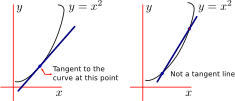
\includegraphics[height=4cm]{tang1}
\end{center}
\end{fig}
Here we have drawn two very rough sketches of the curve $y=x^2$ for $x \geq 0$.
These are not very good sketches for a couple of reasons
\begin{itemize}
 \item The curve in the figure does not pass through $(0,0)$, even though
$(0,0)$ lies on $y=x^2$.
 \item The top-right end of the curve doubles back on itself and so fails the
vertical line test  that all functions must satisfy\footnote{Take a moment to
go back and reread Definition~\ref{def function}.} --- for each $x$-value there
is exactly one $y$-value for which $(x,y)$ lies on the curve $y=x^2$.
\end{itemize}
So let's draw those more carefully.
\begin{fig}
\begin{center}
 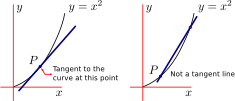
\includegraphics[height=4cm]{tang1a}
\end{center}
{Sketches of the curve $y=x^2$. (left) shows a tangent line, while
(right) shows a line that is not a tangent.}
\label{fig tang1a}
\end{fig}
These are better. In both cases we have drawn $y=x^2$ (carefully) and then
picked a point on the curve --- call it $P$. Let us zoom in on the ``good''
example:
\begin{fig}
\begin{center}
 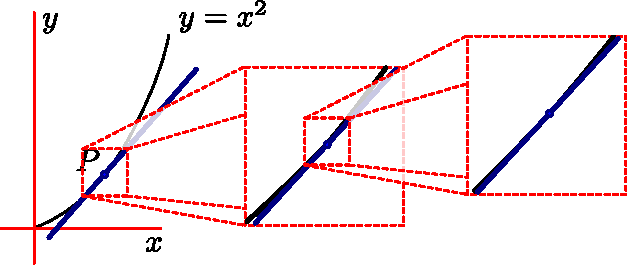
\includegraphics[height=4cm]{tang1aa}
\end{center}
We see that, the more we zoom in on the point $P$, the more the graph of the function
(drawn in black) looks like a straight line --- that line is the tangent line (drawn in
blue).
\label{fig tang1aa}
\end{fig}
We see that as we zoom in on the point $P$, the graph of the function looks
more and more like a straight line. If we kept on zooming in on $P$ then the
graph of the function would be indistinguishable from a straight line. That
line is the tangent line (which we have drawn in blue). A little more
precisely, the blue line is ``the tangent line to the function at $P$''. We
have to be a little careful, because if we zoom in at a different point, then
we will find a different tangent line.

Now let's zoom in on the ``bad'' example we see that the blue line looks very
different from the function; because of this, the blue line is not the tangent
line at $P$.
\begin{fig}
\begin{center}
 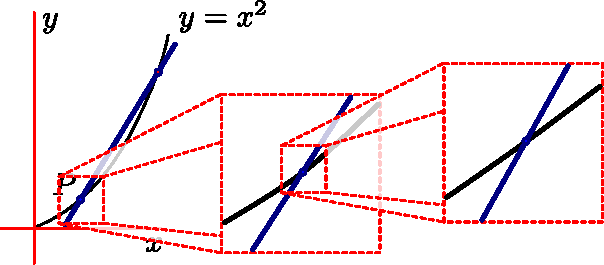
\includegraphics[height=4cm]{tang1ab}
\end{center}
Zooming in on $P$ we see that the function (drawn in black) looks more
and more like a straight line --- however it is not the same line as that drawn
in blue. Because of this the blue line is not the tangent line.
\label{fig tang1ab}
\end{fig}

Here are a couple more examples of tangent lines
\begin{fig}
\begin{center}
 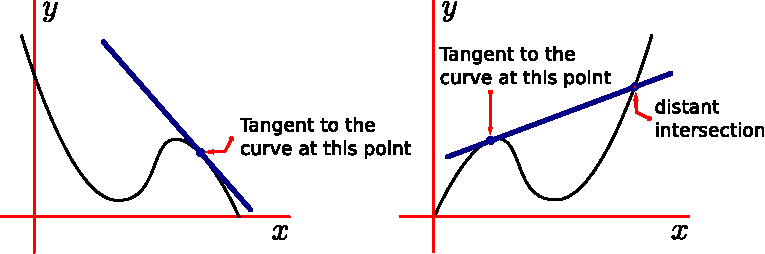
\includegraphics[height=4cm]{tang1b}
\end{center}
More examples of tangent lines.
\label{fig tang1b}
\end{fig}
The one on the left is very similar to the good example on $y=x^2$ that we saw
above, while the one on the right is different --- it looks a little like the
``bad'' example, in that it crosses our function the curve at some distant
point. Why is the line in Figure~\ref{fig tang1b}(right) a tangent while the
line in Figure~\ref{fig tang1a}(right) not a tangent? To see why, we should
again zoom in close to the point where we are trying to draw the tangent.
\begin{fig}
\begin{center}
 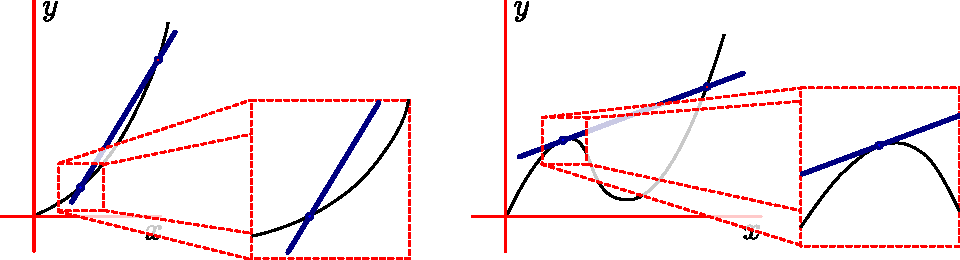
\includegraphics[height=4cm]{tang1c}
\end{center}
\end{fig}
As we saw above in Figure~\ref{fig tang1ab}, when we zoom in around our example
of ``not a tangent line'' we see that the straight line looks very different
from the curve at the ``point of tangency'' --- i.e. where we are trying to draw
the tangent. The line drawn in Figure~\ref{fig tang1b}(right) looks more and
more like the function as we zoom in.

This example raises an important point --- when we are trying to draw a
tangent line, we don't care what the function does a long way from the
point; the tangent line to the curve at a particular point $P$, depends only on
what the function looks like close to that point $P$.

To illustrate this consider the sketch of the function $y = \sin(x)$ and its
tangent line at~$(x,y)=(0,0)$:
\begin{fig}
\begin{center}
 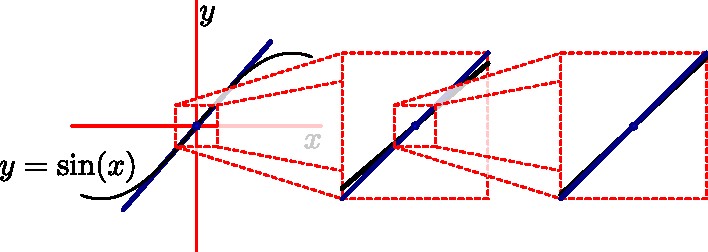
\includegraphics[height=4cm]{tang1d}
\end{center}
\end{fig}
As we zoom in, the graph of $\sin(x)$ looks more and more like a straight line
--- in fact it looks more and more like the line $y=x$. We have also sketched
this tangent line. What makes this example a little odd is that the tangent
line crosses the function. In the examples above, our tangent lines just
``kissed'' the curve and did not cross it (or at least did not cross it
nearby).

Using this idea of zooming in at a particular point, drawing a tangent line is
not too hard. However,  finding the equation of the tangent line presents us
with a few challenges. Rather than leaping into the general  theory, let us do a
specific example. Let us find the equation of the tangent line to the curve
$y=x^2$ at the point $P$ with coordinates\footnote{
Note that the \emph{coordinates} $(x,y)$ is an ordered pair of two numbers $x$
and $y$. Traditionally the first number is called the \emph{abscissa} while the
second is the \emph{ordinate}, but these terms are a little archaic. It is now
much more common to hear people refer to the first number as
the \emph{$x$-coordinate} and the second as \emph{$y$-coordinate}.}
$(x,y)=(1,1)$.

To find the equation of a line we either need
\begin{itemize}
 \item the slope of the line and a point on the line, or
 \item two points on the line, from which we can compute the slope via the
formula
\begin{align*}
  m &= \frac{y_2 - y_1}{x_2 - x_1}
\end{align*}
\end{itemize}
and then write down the equation for the line via a formula such as
\begin{align*}
  y &= m \cdot(x - x_1) + y_1.
\end{align*}


We cannot use the first method because we do not know what the slope of the
tangent line should be. To work out the slope we need calculus --- so we'll
be able to use this method once we get to the next chapter on
``differentiation''.

It is not immediately obvious how we can use the second method, since we only
have one point on the curve, namely $(1,1)$. However we can use it to ``sneak
up'' on the answer.  Let's approximate the tangent line, by drawing a line that
passes through $(1,1)$ and some nearby point --- call it $Q$. Here is our
recipe:
\begin{itemize}
 \item We are given the point $P=(1,1)$ and we are told
\begin{quote}
Find the tangent line to the curve $y=x^2$ that passes through $P = (1,1)$.
\end{quote}
 \item We don't quite know how to find a line given just 1 point, however we do
know how to find a line passing through 2 points. So pick another point on the
curves whose coordinates are very close to $P$. Now rather than picking some
actual numbers, I am going to write our second point as $Q = (1+h, (1+h)^2)$.
That is, a point $Q$ whose $x$-coordinate is equal to that of $P$ plus a little
bit --- where the little bit is some small number $h$.  And since this point
lies on the curve $y=x^2$, and $Q$'s x-coordinate is $1+h$, $Q$'s y-coordinate must
be $(1+h)^2$.

If having $h$ as an variable rather than a number bothers you, start by
thinking of $h$ as~$0.1$.

 \item A picture of the situation will help.
\end{itemize}
\begin{fig}
  \begin{center}
  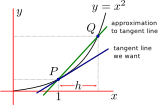
\includegraphics[height=5cm]{tang2}
  \end{center}
\end{fig}
\begin{itemize}
  \item This line that passes through the curve in two places $P$ and $Q$ is
  called a ``secant line''.

  \item The slope of the line is then
\begin{align*}
  m &= \frac{y_2 - y_1}{x_2-x_1} \\
  &= \frac{(1+h)^2-1}{(1+h)-1}
  =  \frac{1+2h+h^2-1}{h}
  = \frac{2h+h^2}{h}
  = 2+h
\end{align*}
  where we have expanded $(1+h)^2 = 1+2h+h^2$ and then cleaned up a bit.
\end{itemize}
Now this isn't our tangent line because it passes through 2 nearby points on
the curve --- however it is a reasonable approximation of it. Now we can make
that approximation better and so ``sneak up'' on the tangent line by considering
what happens when we move this point $Q$ closer and closer to $P$. i.e. make the
number $h$ closer and closer to zero.
\begin{fig}
\begin{center}
  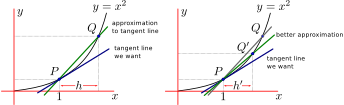
\includegraphics[width=\textwidth]{tang2a}
\end{center}
\end{fig}

First look at the picture. The original choice of $Q$ is on the left, while on
the right we have drawn what happens if we choose $h'$ to be some number a
little smaller than $h$, so that our point $Q$ becomes a new point $Q'$ that is
a little closer to $P$. The new approximation is better than the first.

So as we make $h$ smaller and smaller, we bring $Q$ closer and closer to
$P$, and make our secant line a better and better approximation of the
tangent line. We can observe what happens to the slope of the line as we
make $h$ smaller by plugging some numbers into our formula $m=2+h$:
\begin{align*}
 h=0.1 && m = 2.1\\
 h=0.01 && m= 2.01 \\
 h=0.001 && m= 2.001.
\end{align*}
So again we see that as this difference in $x$ becomes smaller and smaller, the
slope appears to be getting closer and closer to $2$. We can write this more
mathematically as
\begin{align*}
 \lim_{h \to 0} \frac{(1+h)^2-1}{h} &= 2
 \end{align*}
This is read as
\begin{quote}
 The limit, as $h$ approaches $0$, of $\frac{(1+h)^2-1}{h}$ is $2$.
\end{quote}
This is our first limit! Notice that we can see this a little more clearly with a quick
bit of algebra:
\begin{align*}
\frac{(1+h)^2-1}{h} &= \frac{(1+2h+h^2)-1}{h} \\
  &= \frac{2h+h^2}{h} \\
  &= 2+h
\intertext{So it is not unreasonable to expect that}
\lim_{h \to 0} \frac{(1+h)^2-1}{h} &= \lim_{h \to 0} (2+h) = 2.
\end{align*}


Our tangent line can be thought of as the end of this process --- namely as we
bring $Q$ closer and closer to $P$, the slope of the secant line comes
closer and closer to that of the tangent line we want. Since we have worked out
what the slope is --- that is the limit we saw just above --- we now know
the slope of the tangent line is $2$. Given this, we can work out the
equation for the tangent line.
\begin{itemize}
 \item The equation for the line is $y=mx+c$. We have 2 unknowns $m$ and $c$ ---
so we need 2 pieces of information to find them.
 \item Since the line is tangent to $P = (1,1)$ we know the line must pass
through $(1,1)$. From the limit we computed above, we also know that the line
has slope $2$.
 \item Since the slope is $2$ we know that $m=2$. Thus the equation of the line
is $y=2x+c$.
 \item We know that the line passes through $(1, 1)$, so that $y=2x+c$ must be $1$
  when $x=1$. So $1 = 2 \cdot 1 + c$, which forces $c = -1$.
\end{itemize}
So our tangent line is $y=2x-1$.

\section{Another Limit and Computing Velocity} \label{sec velocity}
Computing tangent lines is all very well, but what does this have to do with
applications or the ``Real World''? Well - at least initially our use of limits
(and indeed of calculus) is going to be a little removed from real world
applications. However as we go further and learn more about limits and
derivatives we will be able to get closer to real problems and their solutions.

So stepping just a little closer to the real world, consider the following
problem. You drop a ball from the top of a very very tall building. Let $t$ be
elapsed time measured in seconds, and $s(t)$ be the distance the ball has fallen
in metres. So $s(0) = 0$.

\emph{Quick aside:} there is quite a bit going on in the statement of this
problem. We have described the general picture --- tall building, ball, falling
--- but we have also introduced notation, variables and units. These will be
common first steps in applications and are necessary in order to translate a
real world problem into mathematics in a clear and consistent way.


Galileo\footnote{Perhaps one of the most famous experiments in all of physics
is Galileo's leaning tower of Pisa experiment, in which he dropped two balls
of different masses from the top of the tower and observed that the time
taken to reach the ground was independent of their mass. This
disproved Aristotle's assertion that heavier objects fall faster. It is quite
likely that Galileo did not actually perform this experiment. Rather it was a
thought-experiment. However a quick glance at Wikipedia will turn up some
wonderful footage from the Apollo 15 mission showing a hammer and feather being
dropped from equal height hitting the moon's surface at the same time.
Finally, Galileo determined that the speed of falling objects increases at a
constant rate, which is equivalent to the formula stated here, but it is
unlikely that he wrote down an equation exactly as it is here.}
worked out that $s(t)$ is a quadratic function:
\begin{align*}
  s(t) &= 4.9 t^2.
\end{align*}
The question that is posed is
\begin{quote}
 How fast is the ball falling after 1 second?
\end{quote}

Now before we get to answering this question, we should first be a little more
precise. The wording of this question is pretty sloppy for a couple of reasons:
\begin{itemize}
 \item What we do mean by  ``after 1 second''? We know the ball
will move faster and faster as time passes, so after 1 second it does not fall
at one fixed speed.
 \item As it stands a reasonable answer to the question would be just ``really
fast''. If the person asking the question wants a numerical answer it
would be better to ask ``At what speed'' or ``With what velocity''.
\end{itemize}
We should also be careful using the words ``speed'' and ``velocity'' --- they
are not interchangeable.
\begin{itemize}
 \item Speed means the distance travelled per unit time and is always a
non-negative number. An unmoving object has speed $0$, while a moving object has
positive speed.
 \item Velocity, on the other hand, also specifies the direction of motion.
In this text we will almost exclusively deal with objects moving along
straight lines. Because of this velocities will be positive or negative
numbers indicating  which direction the object is moving along the line. We
will be more precise about this later\footnote{Getting the sign of velocity
wrong is a very common error --- you should be careful with it.}.
\end{itemize}
A better question is
\begin{quote}
 What is the velocity of the ball precisely 1 second after it is dropped?
\end{quote}
or even better:
\begin{quote}
 What is the velocity of the ball at the 1 second mark?
\end{quote}
This makes it very clear that we want to know what is happening at exactly 1
second after the ball is dropped.

There is something a little subtle going on in this question. In particular,
what do we mean by the velocity at $t=1$?. Surely if we freeze time at $t=1$
second, then the object is not moving at all? This is definitely \emph{not}
what we mean.

If an object is moving at a constant velocity\footnote{Newton's first law of
motion states that an object in motion moves with constant velocity unless a
force acts on it --- for example gravity or friction.} in the positive
direction, then that velocity is just the distance travelled divided by the time
taken. That is
\begin{align*}
  v &= \frac{\text{distance moved}}{\text{time taken}}
\end{align*}
An object moving at constant velocity that moves $27$ metres in $3$ seconds has
velocity
\begin{align*}
  v &= \frac{27 m}{3 s} = 9 m/s.
\end{align*}
When velocity is constant everything is easy.

However, in our falling object example, the object is being acted on by
gravity and its speed is definitely not constant. Instead of asking for
\emph{THE} velocity, let us examine the ``average velocity'' of the object over
a certain window of time. In this case the formula is very similar
\begin{align*}
  \text{average velocity } &= \frac{\text{distance moved}}{\text{time taken}}
\end{align*}
But now I want to be more precise, instead write
\begin{align*}
  \text{average velocity } &= \frac{\text{difference in
distance}}{\text{difference in time}}
\end{align*}
Now in spoken English we haven't really changed much --- the distance moved is
the difference in position, and the time taken is just the difference in time
--- but the latter is more mathematically precise, and is easy to translate
into the following equation
\begin{align*}
  \text{average velocity } &= \frac{s(t_2) - s(t_1)}{t_2 - t_1}.
\end{align*}
This is the formula for the average velocity of our object between time $t_1$
and $t_2$. The denominator is just the difference between these times and the
numerator is the difference in position --- i.e. position at time $t_1$ is just
$s(t_1)$ and position at time $t_2$ is just $s(t_2)$.


So what is the average velocity of the falling ball between $1$ and $1.1$
seconds? All we need to do now is plug some numbers into our formula
\begin{align*}
  \mbox{average velocity} &= \frac{\mbox{difference in
position}}{\mbox{difference in time}} \\
  &= \frac{s(1.1) - s(1)}{1.1-1} \\
  &= \frac{4.9 (1.1)^2 - 4.9(1)}{0.1} = \frac{4.9 \times 0.21}{0.1} = 10.29 m/s
\end{align*}
And we have our average velocity. However there is something we should notice
about this formula and it is easier to see if we sketch a graph of the function
$s(t)$
\begin{fig}
\begin{center}
 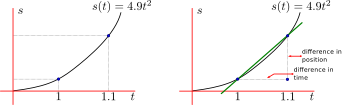
\includegraphics[width=\textwidth]{vel1}
\end{center}
\end{fig}
So on the left I have drawn the graph and noted the times $t=1$ and $t=1.1$.
The
corresponding positions on the axes and the two points on the curve.  On the
right I have added a few more details. In particular I have noted the
differences in position and time, and the line joining the two points. Notice
that the slope of this line is
\begin{align*}
  \text{slope} &= \frac{\text{change in $y$}}{\text{change in $x$}}
  = \frac{\text{difference in $s$}}{\text{difference in $t$}}
\end{align*}
which is precisely our expression for the average velocity.

Let us examine what happens to the average velocity as we look over smaller and
smaller time-windows.
\begin{align*}
  \text{time window} && \text{average velocity}\\
  1 \leq t \leq 1.1 && 10.29 \\
  1 \leq t \leq 1.01 && 9.849 \\
  1 \leq t \leq 1.001 && 9.8049 \\
  1 \leq t \leq 1.0001 && 9.80049
\end{align*}
As we make the time interval smaller and smaller we find that the average
velocity is getting closer and closer to $9.8$. We can be a little more precise
by finding the average velocity between $t=1$ and $t=1+h$ --- this is very
similar to what we did for tangent lines.
\begin{align*}
  \text{average velocity} &= \frac{s(1+h) - s(1)}{(1+h)-1} \\
  &= \frac{4.9(1+h)^2 - 4.9}{h} \\
  &= \frac{9.8h + 4.9h^2}{h} \\
  &= 9.8 + 4.9h
\end{align*}
Now as we squeeze this window between $t=1$ and $t=1+h$ down towards zero, the
average velocity becomes the ``instantaneous velocity'' --- just as the
slope of the secant line becomes the slope of the tangent line. This is
our second limit
\begin{align*}
 v(1) &= \lim_{h \to 0} \frac{s(1+h)-s(1)}{h} = 9.8
\end{align*}
More generally we define the instantaneous velocity at time $t=a$ to be the
limit
\begin{align*}
  v(a) &= \lim_{h \to 0} \frac{ s(a+h) - s(a) }{h}
\end{align*}
We read this as
\begin{quote}
 The velocity at time $a$ is equal to the limit as $h$ goes to zero of
$\frac{s(a+h)-s(a)}{h}$.
\end{quote}

While we have solved the problem stated at the start of this section, it is
clear that if we wish to solve similar problems that we will need to
understand limits in a more general and systematic way.

\section{The Limit of a Function}
\label{sec lim func}

Before we come to definitions, let us start with a little notation for limits.
\begin{notn}\label{ntn_1_3_1}
We will often write
\begin{align*}
  \lim_{x \to a} f(x) = L
\end{align*}
which should be read as
\begin{quote}
The limit of $f(x)$ as $x$ approaches $a$ is $L$.
\end{quote}
\end{notn}
The notation is just shorthand --- we don't want to have to write out long
sentences as we do our mathematics. Whenever you see these symbols you
should think of that sentence.

This shorthand also has the benefit of being mathematically precise (we'll see
this later), and (almost) independent of the language in which the author is
writing. A mathematician who does not speak English can read the above formula
and understand exactly what it means.

In mathematics, like most languages, there is usually more than one way of
writing things and we can also write the above limit as
\begin{align*}
  f(x) \to L \mbox{ as } x \to a
\end{align*}
This can also be read as above, but also as
\begin{quote}
  $f(x)$ goes to $L$ as $x$ goes to $a$
\end{quote}
They mean exactly the same thing in mathematics, even though they might be
written, read and said a little differently.


To arrive at the definition of limit, we want to start\footnote{Well, we
had two limits in the previous sections, so perhaps we really want to
``restart'' with a very simple example.} with a very simple example.

\begin{eg}\label{eg_1_3_1}
Consider the following function.
\begin{align*}
 f(x) &= \begin{cases}
          2x & x<3 \\
          9 & x=3 \\
          2x & x>3
         \end{cases}
\end{align*}
This is an example of a piece-wise function\footnote{We saw another
piecewise function back in Example~\ref{eg piecewise}.}. That is, a function
defined in several pieces, rather than as a single formula. We evaluate the
function at a particular value of $x$ on a case-by-case basis. Here is a sketch
of it
\begin{efig}
\begin{center}
 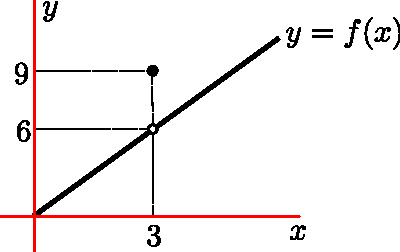
\includegraphics[height=35mm]{piecewise1}
\end{center}
\end{efig}
Notice the two circles in the plot. One is open, $\circ$ and the other is
closed $\bullet$.
\begin{itemize}
 \item A filled circle has quite a precise meaning --- a filled circle at
$(x,y)$ means that the function takes the value $f(x) = y$.
 \item An open circle is a little harder --- an open circle at $(3,6)$ means
that the point $(3,6)$ is not on the graph of $y=f(x)$, i.e. $f(3) \neq 6$.
We should only use the open circle where it is absolutely necessary in order to
avoid confusion.
\end{itemize}
% In the case of our function, for almost all values of $x$ the function is just
% the straight line $y=2x$ --- so we start by drawing that. However at $x=3$
% something different happens and we have $f(3)=9$ --- thus we put a filled
% circle at $(x,y)=(3,9)$. At this point our graph would look like the following
% sketch on the left.
% \begin{center}
%  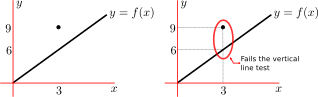
\includegraphics[height=4cm]{piecewise1a}
% \end{center}
% Unfortunately this is not the graph of a function, because it fails the
% vertical line test at $x=3$ --- it appears that $f(3)=9$ and $f(3)=6$ (see the
% sketch on the right). We fix this problem by using an open circle. We place the
% open circle at $(x,y)=(3,6)$ to show that the function is not the continuation
% of the straight line at this point and that in fact $f(3) \neq 6$.


This function is quite contrived, but it is a very good example to start
working with limits more systematically. Consider what the function does close
to $x=3$. We already know what happens exactly at $3$ --- $f(x)=9$ --- but I
want to look at how the function behaves very close to $x=3$. That is, what
does the function do as we look at a point $x$ that gets closer and closer to
$x=3$.

If we plug in some numbers very close to $3$ (but not exactly 3) into the
function we see the following:
\begin{center}
 \begin{tabular}{|c||c|c|c|c|c|c|c|}
  \hline
  $x$ & 2.9 & 2.99 & 2.999 & $\circ$ & 3.001 & 3.01 & 3.1\\
\hline
  $f(x)$ & 5.8 & 5.98 & 5.998 & $\circ$ & 6.002 & 6.02 & 6.2\\
\hline
 \end{tabular}
\end{center}
% \begin{align*}
%   x=2.9 && f(x) = 5.8 \\
%   x=2.99 && f(x) = 5.98 \\
%   x=2.999 && f(x) = 5.998 \\
%   x=3.1 && f(x) = 6.2 \\
%   x=3.01 && f(x) = 6.02 \\
%   x=3.001 && f(x) = 6.002
% \end{align*}
So as $x$ moves closer and closer to 3, without being exactly 3, we see that
the function moves closer and closer to 6. We can write this as
\begin{align*}
  \lim_{x \to 3} f(x) &= 6
\end{align*}
That is
\begin{quote}
 The limit as $x$ approaches $3$ of $f(x)$ is $6$.
\end{quote}
So for $x$ very close to $3$, without being exactly 3, the function is very close to $6$
--- which is a long way from the value of the function exactly at $3$, $f(3)=9$. Note
well that the behaviour of the function as $x$ gets very close to 3 \emph{does not}
depend on the value of the function \emph{at} 3.
\end{eg}

We now have enough to make an informal definition of a limit, which is actually
sufficient for most of what we will do in this text.
\begin{defn}[Informal definition of limit]\label{def_1_3_1}
  We write
\begin{align*}
  \lim_{x \to a} f(x) &= L
\end{align*}
% when the value of the function $f(x)$ gets closer and closer to $L$ as $x$
% gets closer and closer to $a$ (without\footnote{You may find the condition ``without
% being exactly $a$'' a little strange, but there is a good reason for it. One very
% important application of limits, indeed the main reason we teach the topic, is in
% the definition of derivatives (see Definition~\ref{def:DIFFderiv} in the next chapter).
% In that definition we need to compute the limit $\ds \lim_{x\rightarrow
% a}\frac{f(x)-f(a)}{x-a}$. In this case the function whose limit is being taken, namely
% $\frac{f(x)-f(a)}{x-a}$, is not defined at all at $x=a$.} being exactly $a$).
 if the value of the function $f(x)$ is sure to be arbitrarily close to $L$ whenever the value of $x$ is close enough to $a$, without\footnote{You may find the condition ``without  being exactly $a$'' a little strange, but there is a good reason for it. One very  important application of limits, indeed the main reason we teach the topic, is in the definition of derivatives (see Definition~\ref{def:DIFFderiv} in the next chapter).  In that definition we need to compute the limit $\ds \lim_{x\rightarrow a}\frac{f(x)-f(a)}{x-a}$. In this case the function whose limit is being taken, namely  $\frac{f(x)-f(a)}{x-a}$, is not defined at all at $x=a$.} being exactly $a$.
\end{defn}
In order to make this definition more mathematically correct, we need to
make the idea of ``closer and closer'' more precise --- we do this in
Section~\ref{sec opt formal limit}. It should be emphasised that the
formal definition and the contents of that section are optional
material.

For now, let us use the above definition to examine a more substantial
example.
\begin{eg}\label{eg_1_3_2}
Let $f(x) = \frac{x-2}{x^2+x-6}$ and consider its limit as $x \to 2$.


\begin{itemize}
 \item We are really being asked
  \begin{align*}
    \lim_{x \to 2} \frac{x-2}{x^2+x-6} &= \text{ what?}
  \end{align*}
  \item Now if we try to compute $f(2)$ we get $0/0$ which is
undefined. The function is not defined at that point --- this is a good example
of why we need limits.  We have to sneak up on these places where a function is
not defined (or is badly behaved).

 \item \textbf{VERY IMPORTANT POINT:} the fraction $\frac{0}{0}$ is
\emph{not} $\infty$ and it is not $1$, it is not defined. We cannot ever divide
by zero in normal arithmetic and obtain a consistent and mathematically
sensible answer. If you learned otherwise in high-school, you should quickly
unlearn it.

\item Again, we can plug in some numbers close to $2$ and see what we find
\begin{center}
 \begin{tabular}{|c||c|c|c|c|c|c|c|}
  \hline
  $x$ & 1.9 & 1.99 & 1.999 & $\circ$ & 2.001 & 2.01 & 2.1 \\
  \hline
%   $f(x)$ & 0.2040816327 & 0.2004008016 &0.2000400080
%   & $\circ$ & 0.1999600080 & 0.1996007984 & 0.1960784314 \\
  $f(x)$ & 0.20408 & 0.20040 &0.20004
  & $\circ$ & 0.19996 & 0.19960 & 0.19608 \\
\hline
\end{tabular}
\end{center}
% \begin{align*}
%   x=1.9 && f(x) &= 0.2040816327 \\
%   x=1.99 && f(x) &=  0.2004008016 \\
%   x=1.999 && f(x) &= 0.2000400080 \\
%   x=2.1 && f(x) &= 0.1960784314 \\
%   x=2.01 && f(x) &= 0.1996007984 \\
%   x=2.001 && f(x) &= 0.1999600080
% \end{align*}
\item So it is reasonable to suppose that
\begin{align*}
 \lim_{x \to 2} \frac{x-2}{x^2+x-6} &= 0.2
\end{align*}
\end{itemize}

\end{eg}

The previous two examples are nicely behaved in that the limits we tried to
compute actually exist. We now turn to two nastier examples\footnote{Actually,
they are good examples, but the functions in them are nastier.} in which the
limits we are interested in do not exist.

\begin{eg}[A bad example]
\label{eg sinpix}
Consider the following function $f(x) = \sin( \pi /x )$. Find the limit as $x
\to 0$ of $f(x)$.

We should see something interesting happening close to $x=0$ because $f(x)$ is
undefined there. Using your favourite graph-plotting software you can see that
the graph looks roughly like
\begin{efig}
\begin{center}
 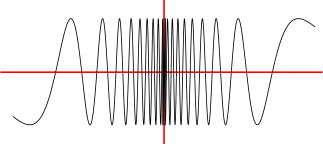
\includegraphics[height=4cm]{lim2}
\end{center}
\end{efig}
How to explain this? As $x$ gets closer and closer to zero, $\pi/x$ becomes
larger and larger (remember what the plot of $y=1/x$ looks like). So when you
take sine of that number, it oscillates faster and faster the closer you get to
zero. Since the function does not approach a single number as we bring $x$
closer and closer to zero, the limit does not exist.

We write this as
\begin{align*}
  \lim_{x\to 0} \sin \left(\frac{\pi}{x}\right) \text{ does not exist}
\end{align*}
It's not very inventive notation, however it is clear. We frequently
abbreviate ``does not exist'' to ``DNE'' and rewrite the above as
\begin{align*}
  \lim_{x\to 0} \sin \left(\frac{\pi}{x}\right) &= \text{DNE}
\end{align*}
\end{eg}

In the following example, the limit we are interested in does not exist.
However the way in which things go wrong is quite different from what we just
saw.
\begin{eg}\label{eg_1_3_3}
Consider the function
\begin{align*}
  f(x) &= \begin{cases}
           x & x<2 \\
           -1 & x=2 \\
           x+3 & x>2
          \end{cases}
\end{align*}
\begin{itemize}
 \item The plot of this function looks like this
\begin{efig}
\begin{center}
 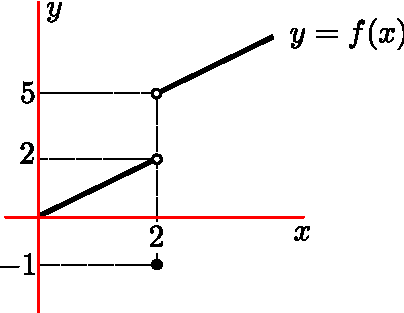
\includegraphics[height=4cm]{lim1}
\end{center}
\end{efig}
\item So let us plug in numbers close to $2$.
\begin{center}
 \begin{tabular}{|c||c|c|c|c|c|c|c|}
  \hline
  $x$ & 1.9 & 1.99 & 1.999 & $\circ$ & 2.001 & 2.01 & 2.1 \\
\hline
  $f(x)$ & 1.9 & 1.99 & 1.999 & $\circ$ & 5.001 & 5.01 & 5.1 \\
\hline
  \end{tabular}
\end{center}
% \begin{align*}
%  x=1.9 && f(x) &= 1.9 \\
%  x=1.99 && f(x) &= 1.99 \\
%  x=1.999 && f(x) &= 1.999 \\
%  x=2.1 && f(x) &= 5.1\\
%  x=2.01 && f(x) &= 5.01\\
%  x=2.001 && f(x) &= 5.001
% \end{align*}
\item This isn't like before. Now when we approach from below, we seem to be
getting closer to $2$, but when we approach from above we seem to be getting
closer to $5$. Since we are not approaching the same number the limit does not
exist.
\begin{align*}
  \lim_{x \to 2} f(x) &= \text{DNE}
\end{align*}
\end{itemize}
\end{eg}

While the limit in the previous example does not exist, the example serves to
introduce the idea of ``one-sided limits''. For example, we can say that
\begin{quote}
 As $x$ moves closer and closer to two \emph{from below} the function
approaches 2.
\end{quote}
and similarly
\begin{quote}
 As $x$ moves closer and closer to two \emph{from above} the function
approaches 5.
\end{quote}

\begin{defn}[Informal definition of one-sided limits]
\label{def informal onesided limits}
We write
\begin{align*}
\lim_{x \to a^-} f(x) &= K
\end{align*}
when the value of $f(x)$ gets closer and closer to $K$ when $x<a$ and $x$ moves
closer and closer to $a$. Since the $x$-values are always less than $a$, we say
that $x$ approaches $a$ \emph{from below}. This is also often called the
left-hand limit since the $x$-values lie to the left of $a$ on a sketch of the
graph.


We similarly write
\begin{align*}
\lim_{x \to a^+} f(x) &= L
\end{align*}
when the value of $f(x)$ gets closer and closer to $L$ when $x>a$ and $x$
moves closer and closer to $a$. For similar reasons we say that $x$ approaches
$a$ from above, and sometimes refer to this as the right-hand limit.
\end{defn}
Note --- be careful to include the superscript $+$ and $-$ when writing
these limits. You might also see the following notations:
\begin{align*}
\lim_{x \to a^+} f(x) &= \lim_{x \to a+} f(x) = \lim_{x \downarrow a} f(x) =
\lim_{x \searrow a} f(x) = L & \text{right-hand limit}\\
\lim_{x \to a^-} f(x) &= \lim_{x \to a-} f(x) = \lim_{x \uparrow a} f(x) =
\lim_{x \nearrow a} f(x) = L & \text{left-hand limit}
\end{align*}
but please use with the notation in Definition~\ref{def informal onesided
limits} above.

Given these two similar notions of limits, when are they the same? The
following theorem tell us
\begin{theorem}[Limits and one sided limits]\label{thm_1_3_1}
\begin{align*}
  \lim_{x \to a} f(x) = L && \mbox{ if and only if }
  && \lim_{x \to a^-} f(x) = L  \mbox{ and }
  \lim_{x \to a^+} f(x) = L
\end{align*}
\end{theorem}
Notice that this is really two separate statements because of the ``if and only
if''
\begin{itemize}
 \item If the limit of $f(x)$ as $x$ approaches $a$ exists and is equal to $L$,
then both the left-hand and right-hand limits exist and are equal to $L$. AND,
 \item If the left-hand and right-hand limits as $x$ approaches $a$ exist and
are equal, then the limit as $x$ approaches $a$ exists and is equal to the
one-sided limits.
\end{itemize}
That is --- the limit of $f(x)$ as $x$ approaches $a$ will only exist if it
doesn't matter which way we approach $a$ (either from left or right)
\emph{AND}
if we get the same one-sided limits when we approach from left and right, then
the limit exists.



We can rephrase the above by writing the contrapositives\footnote{\label{footnote contrapositive}Given a
statement of the form ``If A then B'', the contrapositive is ``If not B then
not A''. They are logically equivalent --- if one is true then so is the
other. We must take care not to confuse the contrapositive with the converse.
Given ``If A then B'', the converse is ``If B then A''. These are definitely not
the same.

To see this consider the statement ``If he is Shakespeare then he is dead.''
The converse is ``If he is dead then he is Shakespeare'' --- clearly garbage
since there are plenty of dead people who are not Shakespeare. The
contrapositive is ``If he is not dead then he is not Shakespeare'' --- which
makes much more sense.} of the above statements.
\begin{itemize}
\item If either of the left-hand and right-hand limits as $x$ approaches $a$
fail to exist, or if they both exist but are different, then the limit as $x$
approaches $a$ does not exist. AND,
 \item If the limit as $x$ approaches $a$ does not exist, then the left-hand
and right-hand limits are either different or at least one of them does not
exist.
\end{itemize}

Here is another limit example
\begin{eg}\label{eg_1_3_4}
Consider the following two functions and compute their limits and one-sided
limits as $x$ approaches 1:
\begin{efig}
\begin{center}
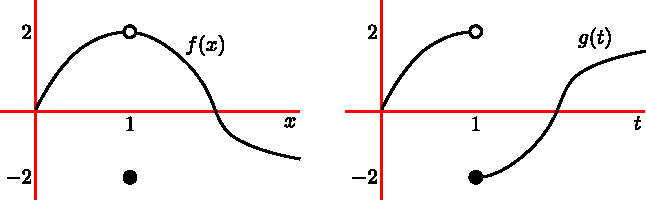
\includegraphics[height=4cm]{lim3}
\end{center}
\end{efig}
These are a little different from our previous examples, in that we do not have
formulas, only the sketch. But we can still compute the limits.
\begin{itemize}
 \item Function on the left --- $f(x)$:
\begin{align*}
  \lim_{x \to 1^-} f(x) &= 2 &
  \lim_{x \to 1^+} f(x) &= 2 \\
\intertext{so by the previous theorem }
\lim_{x \to 1} f(x) &= 2
\end{align*}
 \item Function on the right --- $g(t)$:
\begin{align*}
  \lim_{t \to 1^-} g(t) &= 2
  & \text{and } \lim_{t \to 1^+} g(t) &= -2
\intertext{so by the previous theorem }
  \lim_{t \to 1} g(t) &= \text{DNE}
\end{align*}
\end{itemize}
\end{eg}

We have seen 2 ways in which a limit does not exist --- in one case the
function oscillated wildly, and in the other there was some sort of ``jump'' in
the function, so that the left-hand and right-hand limits were different.

There is a third way that we must also consider. To describe this, consider the
following four functions:
\begin{fig}
\label{fig inf limits}
\begin{center}
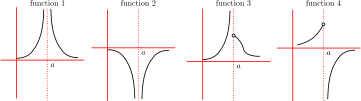
\includegraphics[width = \textwidth]{lim4}
\end{center}
\end{fig}
None of these functions are defined at $x=a$, nor do the limits as $x$
approaches $a$ exist. However we can say more than just ``the limits do not
 exist''.

Notice that the value of function~1 can be made bigger and bigger as we bring
$x$ closer and closer to $a$. Similarly the value of the second function can be
made arbitrarily large and negative (i.e. make it as big a negative number as we
want) by bringing $x$ closer and closer to~$a$. Based on this observation we
have the following definition.
\begin{defn}
\label{def lim is inf informal}
  We write
 \begin{align*}
  \lim_{x \to a} f(x) = + \infty
 \end{align*}
  when the value of the function $f(x)$ becomes arbitrarily large and
  positive as $x$ gets closer and closer to $a$, without being exactly $a$.

  Similarly, we write
 \begin{align*}
  \lim_{x \to a} f(x) = - \infty
 \end{align*}
  when the value of the function $f(x)$ becomes arbitrarily large and
  negative as $x$ gets closer and closer to $a$, without being exactly $a$.
\end{defn}
A good examples of the above is
\begin{align*}
  \lim_{x \to 0} \frac{1}{x^2} &= +\infty
  & \lim_{x \to 0} -\frac{1}{x^2} &= -\infty
\end{align*}
\textbf{IMPORTANT POINT: } Please do not think of ``$+\infty$'' and ``$-\infty$''
in these statements as numbers. You should think of $\lim\limits_{x\rightarrow a} f(x) = +\infty$ and $\lim\limits_{x\rightarrow a} f(x) = -\infty$
as special cases of  $\lim\limits_{x\rightarrow a} f(x) = \text{DNE}$. The statement
\begin{align*}
  \lim_{x \to a} f(x) = +\infty
\end{align*}
does not say ``the limit of $f(x)$ as $x$ approaches $a$ is positive infinity''.
It says ``the function $f(x)$ becomes arbitrarily large as $x$ approaches $a$''.
These are different statements; remember that $\infty$ is not a
number\footnote{One needs to be very careful making statements about
infinity. At some point in our lives we get around to asking ourselves ``what
is the biggest number'', and we realise there isn't one. That is, we can go on
counting integer after integer, for ever and not stop. Indeed the set of
integers is the first infinite thing we really encounter. It is an example of a
\emph{countably infinite} set. The set of real-numbers is actually much bigger
and is \emph{uncountably infinite}. In fact there are an infinite number of
different sorts of infinity! Much of the theory of infinite sets was
developed by Georg Cantor; we mentioned him back in Section~\ref{sec sets} and he is well
worth googling.}.



Now consider functions~3 and~4 in Figure~\ref{fig inf limits}. Here we can make
the value of the function as big and positive as we want (for function~3) or as
big and negative as we want (for function~4) but only when $x$ approaches $a$
from one side. With this in mind we can construct similar notation and a
similar definition:
\begin{defn}
\label{def onesidedlim is inf informal}
  We write
 \begin{align*}
  \lim_{x \to a^+} f(x) = + \infty
 \end{align*}
  when the value of the function $f(x)$ becomes arbitrarily large and
  positive as $x$ gets closer and closer to $a$ from above (equivalently ---
from the right), without being exactly $a$.

  Similarly, we write
 \begin{align*}
  \lim_{x \to a^+} f(x) = - \infty
 \end{align*}
  when the value of the function $f(x)$ becomes arbitrarily large and
  negative as $x$ gets closer and closer to $a$ from above (equivalently ---
from the right), without being exactly $a$.

  The notation
\begin{align*}
  \lim_{x \to a^-} f(x) &= + \infty
&
  \lim_{x \to a^-} f(x) &= - \infty
\end{align*}
  has a  similar meaning except that limits are approached from below / from
the left.
\end{defn}
So for function~3 we have
\begin{align*}
  \lim_{x\to a^-} f(x) &= +\infty
&
  \lim_{x\to a^+} f(x) &= \text{some positive number}
\end{align*}
and for function~4
\begin{align*}
  \lim_{x\to a^-} f(x) &= \text{some positive number}
&
  \lim_{x\to a^+} f(x) &= -\infty
\end{align*}

More examples:
\begin{eg}\label{eg_1_3_5}
Consider the function
\begin{align*}
  g(x) &= \frac{1}{\sin(x)}
\end{align*}
Find the one-sided limits of this function as $x \to \pi$.

Probably the easiest way to do this is to first plot the graph of $\sin(x)$ and
$1/x$ and then think carefully about the one-sided limits:
\begin{efig}
\begin{center}
 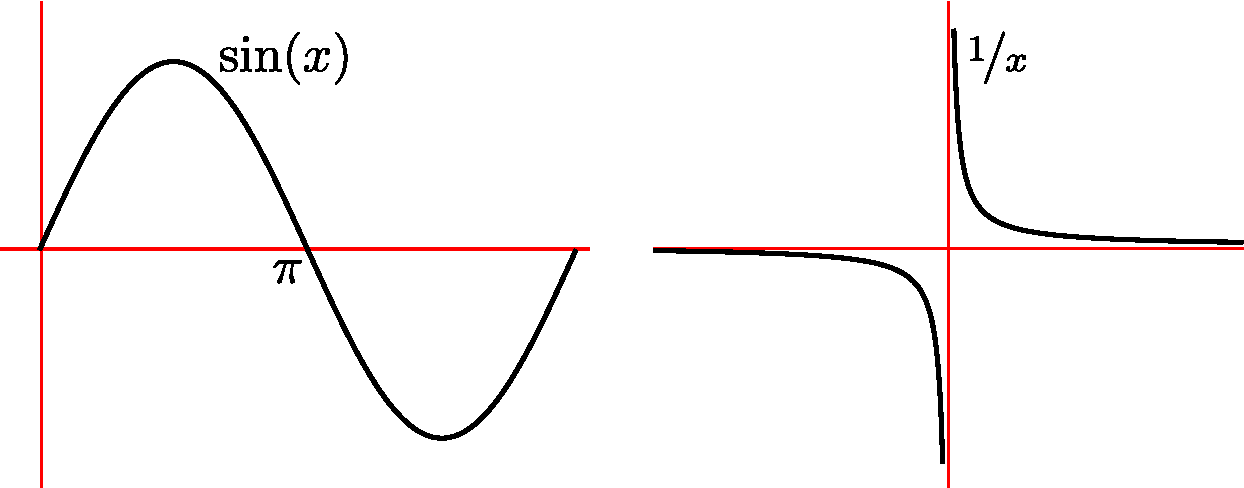
\includegraphics[width=0.8\textwidth]{sinx_1onx}
\end{center}
\end{efig}
\begin{itemize}
 \item As $x \to \pi$ from the left, $\sin(x)$ is a small positive number that
is getting closer and closer to zero. That is, as $x \to \pi^-$, we have that
$\sin(x) \to 0$ through positive numbers (i.e. from above). Now look at the graph
of $1/x$, and think what happens as we move $x \to 0^+$, the function is
positive and becomes larger and larger.

So as $x \to \pi$ from the left, $\sin(x) \to 0$ from above, and so $1/\sin(x)
\to +\infty$.

\item By very similar reasoning, as $x \to \pi$ from the right, $\sin(x)$ is a
small negative number that gets closer and closer to zero. So as $x \to \pi$
from the right, $\sin(x) \to 0$ through negative numbers (i.e. from below) and so
$1/\sin(x)$ to $-\infty$.
\end{itemize}
Thus
\begin{align*}
  \lim_{x \to \pi^-} \frac{1}{\sin(x)} &= +\infty &
  \lim_{x \to \pi^+} \frac{1}{\sin(x)} &= -\infty
\end{align*}
\end{eg}


Again, we can make Definitions~\ref{def lim is inf informal}
and~\ref{def onesidedlim is inf informal} into mathematically precise formal
definitions using techniques very similar to those in the optional
Section~\ref{sec opt formal limit}. This is not strictly necessary for this
course.

Up to this point we explored limits by sketching graphs or plugging values into
a calculator. This was done to help build intuition, but it is not really the
basis of a systematic method for computing limits. We have also avoided more
formal approaches\footnote{The formal
approaches are typically referred to as ``epsilon-delta limits'' or
``epsilon-delta proofs'' since the symbols $\epsilon$ and $\delta$ are
traditionally used throughout. Take a peek at Section~\ref{sec opt
formal limit} to see.} since we do not have time in the course to go into
that level of detail and (arguably) we don't need that detail to achieve the
aims of the course. Thankfully we can develop a more systematic approach based
on the idea of building up complicated limits from simpler ones by examining how
limits interact with the basic operations of arithmetic.

\section{Calculating Limits with Limit Laws}\label{sec_1_4}
Think back to the functions you know and the sorts of things you have  been
asked to draw, factor and so on. Then they are all constructed from simple
pieces, such as
\begin{itemize}
 \item constants --- $c$
 \item monomials --- $x^n$
 \item trigonometric functions --- $\sin(x), \cos(x)$ and $\tan(x)$
\end{itemize}
These are the building blocks from which we construct functions. Soon we will
add a few more functions to this list, especially the exponential function and
various inverse functions.

We then take these building blocks and piece them together using arithmetic
\begin{itemize}
 \item addition and subtraction --- $f(x)  = g(x) + h(x)$ and $f(x) = g(x) -
h(x)$
 \item multiplication --- $f(x) = g(x) \cdot h(x)$
 \item division --- $f(x) = \frac{g(x)}{h(x)}$
 \item substitution --- $f(x) = g( h(x) )$ --- this is also called
the composition of $g$ with $h$.
\end{itemize}
The idea of building up complicated functions from simpler pieces was discussed
in Section~\ref{sec parsing}.

What we will learn in this section is how to compute the limits of the basic
building blocks and then how we can compute limits of sums, products and so
forth using ``limit laws''. This process allows us to compute limits of
complicated functions, using very simple tools and without having to resort to
``plugging in numbers'' or ``closer and closer'' or ``$\epsilon-\delta$
arguments''.


In the examples we saw above, almost all the \emph{interesting} limits happened
at points where the underlying function was badly behaved --- where it jumped,
was not defined or blew up to infinity. In those cases we had to be careful and
think about what was happening. Thankfully most functions we will see do not
have too many points at which these sorts of things happen.

For example, polynomials do not have any nasty jumps and are defined everywhere
and do not ``blow up''. If you plot them, they look smooth\footnote{We have
used this term in an imprecise way, but it does have a precise
mathematical meaning.}. Polynomials and limits behave very nicely together,
and for any polynomial $P(x)$ and any real number $a$ we have that
\begin{align*}
  \lim_{x \to a} P(x) &= P(a)
\end{align*}
That is --- to evaluate the limit we just plug in the number. We will build up
to this result over the next few pages.

Let us start with the two easiest limits\footnote{Though it lies outside the
scope of the course, you can find the formal $\epsilon$-$\delta$ proof of this
result at the end of Section~\ref{sec opt formal limit}.}
\begin{theorem}[Easiest limits]\label{thm_easy_lim}
\label{thm easy lim}
   Let $a,c \in \mathbb{R}$. The following two limits hold
  \begin{align*}
  \lim_{x \to a} c & = c & \text{ and }&&
  \lim_{x \to a} x &= a.
\end{align*}
\end{theorem}

Since we have not seen too many theorems yet, let us examine it carefully piece
by piece.
\begin{itemize}
 \item \textbf{Let $a,c \in \mathbb{R}$} --- just as was the case for
definitions, we start a theorem by defining terms and setting the scene. There
is not too much scene to set: the symbols $a$ and $c$ are real numbers.
 \item \textbf{The following two limits hold} --- this doesn't really
contribute much to the statement of the theorem, it just makes it easier to
read.
 \item $\ds \mathbf{\lim_{x \to a} c  = c}$  --- when we take the
limit of a
constant function (for example think of $c=3$), the limit is (unsurprisingly)
just that same constant.
 \item $\ds \mathbf{\lim_{x \to a} x = a}$ --- as we noted above for general
polynomials, the limit of the function $f(x) = x$ as $x$ approaches a given
point $a$, is just $a$. This says something quite obvious --- as $x$ approaches
$a$, $x$ approaches $a$ (if you are not convinced then sketch the graph).
\end{itemize}


Armed with only these two limits, we cannot do very much. But combining these
limits with some arithmetic we can do quite a lot. For a moment, take a step
back from limits for a moment and think about how we construct functions. To
make the discussion a little more precise think about how we might construct
the function
\begin{align*}
  h(x) &= \frac{2x-3}{x^2+5x-6}
\end{align*}

If we want to compute the value of the function at
$x=2$, then we would
\begin{itemize}
 \item compute the numerator at $x=2$
 \item compute the denominator at $x=2$
 \item compute the ratio
\end{itemize}
Now to compute the numerator we
\begin{itemize}
 \item take $x$ and multiply it by 2
 \item subtract 3 to the result
\end{itemize}
While for the denominator
\begin{itemize}
 \item multiply $x$ by $x$
 \item multiply $x$ by 5
 \item add these two numbers and subtract $6$
\end{itemize}
This sequence of operations can be represented pictorially
as the tree shown in Figure~\ref{fig parse me} below.
\begin{fig}
\label{fig parse me}
 \begin{center}
  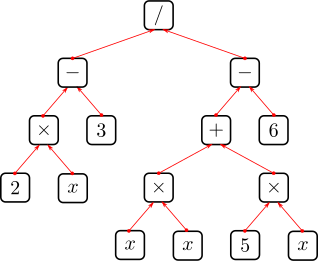
\includegraphics[scale=0.5]{tree3}
 \end{center}
\end{fig}
Such trees were discussed in Section~\ref{sec parsing} (now is not a bad time to quickly
review that section before proceeding). The point here is that in order to compute the
value of the function we just repeatedly add, subtract, multiply and divide constants and
$x$.


To compute the limit of the above function at $x=2$ we can do something very
similar. From the previous theorem we know how to compute
\begin{align*}
  \lim_{x \to 2} c &= c && \text{and} & \lim_{x \to 2} x &= 2
\end{align*}
and the next theorem will tell us how to stitch together these two limits using
the arithmetic we used to construct the function.

\begin{theorem}[Arithmetic of limits]\label{thm arith lim}
  Let $a,c \in \mathbb{R}$, let $f(x)$ and $g(x)$ be defined for all $x$'s that lie in
some interval about $a$ (but $f,g$ need not be defined exactly at $a$).
 \begin{align*}
  \lim_{x \to a} f(x)&=F & \lim_{x \to a} g(x) &=G
\end{align*}
  exist with $F,G \in \mathbb{R}$. Then the following limits hold
\begin{itemize}
 \item $\ds \lim_{x \to a} ( f(x) + g(x) ) = F+G$ --- limit of the sum is the
sum of the limits.
 \item $\ds \lim_{x \to a} ( f(x) - g(x) ) = F - G$ --- limit of the difference
is the difference of the limits.
\item $\ds \lim_{x \to a} c f(x) = c F$.
\item $\ds \lim_{x \to a} ( f(x) \cdot g(x) ) = F \cdot G$ --- limit of
the product is the product of limits.
\item If $G \neq 0$ then $\ds \lim_{x \to a} \frac{f(x)}{g(x)} = \frac{F}{G}$
and, in particular,
             $\ds \lim_{x\rightarrow a}\frac{1}{g(x)}=\frac{1}{G}$.
\end{itemize}
Note --- be careful with this last one --- the denominator cannot be zero.
\end{theorem}
The above theorem shows that limits interact very simply with arithmetic. If
you are asked to find the limit of a sum then the answer is just the sum of the
limits. Similarly the limit of a product is just the product of the limits.


How do we apply the above theorem to the rational function $h(x)$ we defined
above? Here is a warm-up example:
\begin{eg}\label{eg_1_4_1}
You are given two functions $f,g$ (not explicitly) which have the following
limits as $x$ approaches 1:
\begin{align*}
  \lim_{x \to 1} f(x)&=3 && \text{and} & \lim_{x\to 1} g(x)&=2
\end{align*}
Using the above theorem we can compute
\begin{align*}
 \lim_{x \to 1} 3f(x) &= 3 \times 3 = 9 \\
 \lim_{x \to 1} 3f(x) -g(x) &= 3\times 3 -2 = 7\\
 \lim_{x \to 1} f(x) g(x) &= 3\times 2 = 6\\
 \lim_{x \to 1} \frac{f(x)}{f(x) -g(x)} &= \frac{3}{3-2} = 3
\end{align*}
\end{eg}

Another simple example
\begin{eg}\label{eg_1_4_2}
 Find $\ds \lim_{x \to 3} 4x^2-1$

 We use the arithmetic of limits:
\begin{align*}
  \lim_{x \to 3} 4x^2-1
  &= \left( \lim_{x \to 3} 4x^2 \right) - \lim_{x \to 3} 1
  & \text{difference of limits}
\\
  &= \left( \lim_{x \to 3} 4  \cdot \lim_{x \to 3} x^2 \right) -  \lim_{x \to
3} 1
  & \text{product of limits} \\
  &= 4 \cdot \left( \lim_{x \to 3} x^2 \right) -  1
  & \text{limit of constant} \\
  &= 4 \cdot \left( \lim_{x \to 3} x \right) \cdot \left( \lim_{x \to 3} x
\right)-1
  & \text{product of limits} \\
  &= 4 \cdot 3 \cdot 3 - 1
  & \text{limit of $x$} \\
  &= 36 - 1 \\
  &= 35
\end{align*}
\end{eg}
This is an excruciating level of detail, but when you first use this theorem
and try some examples it is a good idea to do things step by step by step until
you are comfortable with it.
\begin{eg}\label{eg_1_4_3}
Yet another limit --- compute $\ds \lim_{x\to 2} \frac{x}{x-1}$.

To apply the arithmetic of limits, we need to examine numerator and
denominator separately and make sure the limit of the denominator is non-zero.
Numerator first:
\begin{align*}
  \lim_{x \to 2} x & = 2 & \text{limit of $x$}
\intertext{and now the denominator:}
  \lim_{x \to 2} x-1
  & = \left( \lim_{x \to 2} x \right) - \left( \lim_{x \to 2} 1 \right)
  & \text{difference of limits} \\
  & = 2 - 1
  & \text{limit of $x$ and limit of constant}
  & = 1
\end{align*}
Since the limit of the denominator is non-zero we can put it back together to
get
\begin{align*}
  \lim_{x\to 2} \frac{x}{x-1} &= \frac{\ds \lim_{x\to 2} x}{\ds \lim_{x \to
2}(x-1)}  \\
  &= \frac{2}{1} \\
  &= 2
\end{align*}
\end{eg}

In the next example we show that many different things can happen if
the limit of the denominator is zero.
\begin{eg}[Be careful with limits of ratios]\label{eg lim rat}
We must be careful when computing the limit of a ratio --- it
is the ratio of the limits except when the limit of the denominator is zero.
When the limit of the denominator is zero Theorem~\ref{thm arith lim}
\textbf{does not apply} and a few interesting things can happen
\begin{itemize}
 \item If the limit of the numerator is non-zero then the limit of the ratio
does not exist
\begin{align*}
  \lim_{x \to a} \frac{f(x)}{g(x)} &= DNE & \text{when $\lim_{x\to a} f(x) \neq
0$ and $\lim_{x \to a} g(x)=0$}
\end{align*}
  For example, $\ds \lim_{x \to 0} \frac{1}{x^2} = DNE$.
 \item If the limit of the numerator is zero then the above theorem does not
give us enough information to decide whether or not the limit exists. It is
possible that
\begin{itemize}
 \item the limit does not exist, eg. $\ds \lim_{x \to 0} \frac{x}{x^2} =
\lim_{x
\to 0} \frac{1}{x} = DNE$
 \item the limit is $\pm \infty$, eg. $\ds \lim_{x \to 0} \frac{x^2}{x^4} =
\lim_{x
\to 0} \frac{1}{x^2} = +\infty$ or $\ds \lim_{x \to 0} \frac{-x^2}{x^4} =
\lim_{x\to 0} \frac{-1}{x^2} = -\infty$.
 \item the limit is zero, eg. $\ds \lim_{x \to 0} \frac{x^2}{x} = 0$
 \item the limit exists and is non-zero, eg. $\ds \lim_{x \to 0} \frac{x}{x} =
1$
\end{itemize}
\end{itemize}
Now while the above examples are very simple and a little contrived they serve
to illustrate the point we are trying to make --- be careful if the limit of
the denominator is zero.
\end{eg}



We now have enough theory to return to our rational function and compute its
limit as $x$ approaches 2.
\begin{eg}\label{eg_1_4_4}
 Let $\ds h(x) = \frac{2x-3}{x^2+5x-6}$ and find its limit as $x$ approaches
$2$.

Since this is the limit  of a ratio, we compute the limit of the numerator and
denominator separately.
Numerator first:
\begin{align*}
  \lim_{x \to 2} 2x-3
  &= \left( \lim_{x \to 2} 2x \right) - \left( \lim_{x \to 2} 3 \right)
  & \text{difference of limits} \\
  &= 2 \cdot \left( \lim_{x \to 2} x \right) -3
  & \text{product of limits and limit of constant} \\
  &= 2 \cdot 2 -3
  & \text{limits of $x$} \\
  &= 1
\end{align*}
Denominator next:
\begin{align*}
  \lim_{x \to 2} x^2+5x-6
  &= \left( \lim_{x \to 2} x^2 \right) + \left( \lim_{x \to 2} 5x \right)
  - \left( \lim_{x \to 2} 6 \right)
  & \text{sum of limits} \\
  &= \left( \lim_{x \to 2} x \right)\cdot \left( \lim_{x \to 2} x \right)
  + 5 \cdot \left( \lim_{x \to 2} x \right) - 6
  & \text{product of limits and limit of constant} \\
  &= 2 \cdot 2 + 5 \cdot 2 - 6
  & \text{limits of $x$} \\
  &= 8
\end{align*}
Since the limit of the denominator is non-zero, we can obtain our result by
taking the ratio of the separate limits.
\begin{align*}
\lim_{x \to 2} \frac{2x-3}{x^2+5x-6}
  &= \frac{\ds \lim_{x \to 2} 2x-3}{\ds \lim_{x \to 2} x^2+5x-6} = \frac{1}{8}
\end{align*}

The above works out quite simply. However, if we were to take the limit as $x
\to 1$ then things are a bit harder. The limit of the numerator is:
\begin{align*}
  \lim_{x \to 1} 2x-3 &= 2 \cdot 1 - 3 = -1
\end{align*}
(we have not listed all the steps). And the limit of the denominator is
\begin{align*}
  \lim_{x \to 1} x^2 +5x-6 &= 1 \cdot 1 + 5 - 6 = 0
\end{align*}
Since the limit of the numerator is non-zero, while the limit of the
denominator is zero, the limit of the ratio does not exist.
\begin{align*}
\lim_{x \to 1} \frac{2x-3}{x^2+5x-6}
  &= DNE
\end{align*}
\end{eg}
It is \textbf{IMPORTANT TO NOTE} that it is not correct to write
\begin{align*}
\lim_{x \to 1} \frac{2x-3}{x^2+5x-6}
  &= \frac{-1}{0} = DNE
\end{align*}
Because we can only write
\begin{align*}
  \lim_{x \to a} \frac{f(x)}{g(x)} &= \frac{\ds \lim_{x \to a} f(x)}{\ds
\lim_{x \to a} g(x) } = \text{something}
\end{align*}
when the limit of the denominator is non-zero (see Example~\ref{eg lim rat} above).

With a little care you can use the arithmetic of limits to obtain the
following rules for limits of powers of functions and limits of roots of
functions:
\begin{theorem}[More arithmetic of limits --- powers and roots]
\label{thm lim powers}
  Let $n$ be a positive integer, let $a \in \mathbb{R}$ and let $f$ be a
function so that
\begin{align*}
  \lim_{x \to a} f(x) &= F
\end{align*}
  for some real number $F$. Then the following holds
\begin{align*}
  \lim_{x \to a} \left( f(x) \right)^n
  &= \left(\lim_{x \to a} f(x) \right)^n = F^n
\end{align*}
so that the limit of a power is the power of the limit. Similarly, if
\begin{itemize}
 \item $n$ is an even number and $F>0$, or
 \item $n$ is an odd number and $F$ is any real number
\end{itemize}
then
\begin{align*}
  \lim_{x \to a} \left( f(x) \right)^{1/n}
  &= \left(\lim_{x \to a} f(x) \right)^{1/n} = F^{1/n}
\end{align*}
More generally\footnote{You may not know the definition of the power
$b^p$ when $p$ is not a rational number, so here it is. If $b>0$ and $p$
is any real number, then $b^p$ is the limit of $b^r$ as $r$ approaches $p$ 
through rational numbers. We won't do so here, but it is possible to prove that the limit exists.}, if $F>0$ and $p$ is any real number,
\begin{align*}
  \lim_{x \to a} \left( f(x) \right)^p
  &= \left(\lim_{x \to a} f(x) \right)^p = F^p
\end{align*}
\end{theorem}
Notice that we have to be careful when taking roots of limits that might be
negative numbers. To see why, consider the case $n=2$, the limit
\begin{align*}
  \lim_{x \to 4} x^{1/2} &= 4^{1/2} = 2 \\
  \lim_{x \to 4} (-x)^{1/2} &= (-4)^{1/2} = \text{not a real number}
\end{align*}
In order to evaluate such limits properly we need to use complex numbers which
are beyond the scope of this text.

Also note that the notation $x^{1/2}$ refers to the \emph{positive} square root
of $x$. While $2$ and $(-2)$ are both square-roots of $4$, the notation
$4^{1/2}$ means $2$. This is something we must be careful of\footnote{Like
ending sentences in prepositions --- ``This is something up with which we will
not put.'' This quote is attributed to Churchill though there is some dispute as to
whether or not he really said it.}.

So again --- let us do a few examples and carefully note what we are doing.
\begin{eg}\label{eg_1_4_5}
\begin{align*}
  \lim_{x \to 2} (4x^2-3)^{1/3} &=
  \left( (\lim_{x\to 2} 4x^2) - (\lim_{x \to 2} 3) \right)^{1/3} \\
  &= \left( 4 \cdot 2^2  - 3 \right)^{1/3}\\
  &= \left( 16-3 \right)^{1/3} \\
  &= 13^{1/3}
\end{align*}
\end{eg}

By combining the last few theorems we can make the evaluation of limits of
polynomials and rational functions much easier:
\begin{theorem}[Limits of polynomials and rational functions]\label{thm_1_4_1}
Let $a \in \mathbb{R}$, let $P(x)$ be a polynomial and let $R(x)$ be a rational
function. Then
\begin{align*}
  \lim_{x \to a} P(x) &= P(a)
\end{align*}
and provided $R(x)$ is defined at $x=a$ then
\begin{align*}
  \lim_{x \to a} R(x) &= R(a)
\end{align*}
If $R(x)$ is not defined at $x=a$ then we are not able to apply this result.
\end{theorem}
So the previous examples are now much easier to compute:
\begin{align*}
\begin{array}{rcccr}
  \ds\lim_{x \to 2} \frac{2x-3}{x^2+5x-6} &=& \ds \frac{4-3}{4+10-6} &=&
\ds \frac{1}{8}\\[3ex]
  \ds\lim_{x\to 2} (4x^2-1) &=& 16-1 &=& 15 \\[1ex]
  \ds\lim_{x\to 2} \frac{x}{x-1} &=& \ds \frac{2}{2-1} &=& 2
\end{array}
\end{align*}


It is clear that limits of polynomials are very easy, while those of rational
functions are easy except when the denominator might go to zero. We have seen
examples where the resulting limit does not exist, and some where it does. We
now work to explain this more systematically. The following example demonstrates that it
is sometimes possible to take the limit of a rational function to a point at which the
denominator is zero. Indeed we must be able to do exactly this in order to be able to
define derivatives in
the next chapter.
\begin{eg}\label{eg zero cancel limit}
Consider the limit
\begin{align*}
    \lim_{x \to 1} \frac{x^3-x^2}{x-1}.
\end{align*}
If we try to apply the arithmetic of limits then we compute the limits of the
numerator and denominator separately
\begin{align}
    \lim_{x \to 1} x^3-x^2 &= 1-1 = 0 \\
    \lim_{x \to 1} x-1 &= 1-1 = 0
\end{align}
Since the denominator is zero, we cannot apply our theorem and we are, for the
moment, stuck. However, there is more that we can do here --- the hint is that
the numerator and denominator \emph{both} approach zero as $x$ approaches 1. This
means that there might be something we can cancel.

So let us play with the expression a little more before we take the limit:
\begin{align*}
  \frac{x^3-x^2}{x-1} &= \frac{x^2(x-1)}{x-1} = x^2
  & \text{ provided $x \neq 1$.}
\end{align*}
So what we really have here is the following function
\begin{align*}
  \frac{x^3-x^2}{x-1} &= \begin{cases}
                          x^2 & x \neq 1 \\
                          \text{undefined } & x = 1
                         \end{cases}
\end{align*}
If we plot the above function the graph looks exactly the same as $y=x^2$
except that the function is not defined at $x=1$ (since at $x=1$ both numerator and
denominator are zero).
\begin{efig}
\begin{center}
 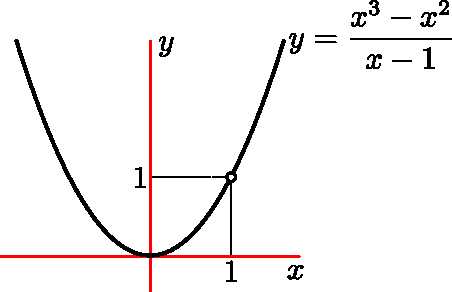
\includegraphics[height=4cm]{rat1}
\end{center}
\end{efig}
When we compute a limit as $x \to a$, the value of the function exactly at
$x=a$ is irrelevant. We only care what happens to the function as we bring $x$
very close to $a$. So for the above problem we can write
\begin{align*}
    \frac{x^3-x^2}{x-1} &= x^2 & \text{when $x$ is close to $1$ but not at
$x=1$}
\end{align*}
So the limit as $x \to 1$ of the function is the same as the limit $\ds \lim_{x\to
1} x^2$ since the functions are the same except exactly at $x=1$. By this
reasoning we get
\begin{align*}
    \lim_{x \to 1} \frac{x^3-x^2}{x-1} &=
    \lim_{x \to 1} x^2 = 1
\end{align*}
\end{eg}
The reasoning in the above example can be made more general:
\begin{theorem}\label{thm_1_4_2}
 If $f(x) = g(x)$ except when $x=a$ then $\ds \lim_{x\to a} f(x) = \lim_{x\to
a}
g(x)$ provided the limit of $g$ exists.
\end{theorem}

How do we know when to use this theorem? The big clue is that when we try to
compute the limit in a naive way, we end up with $\frac{0}{0}$. We know that
$\frac{0}{0}$ does not make sense, but it is an indication that there might be a
common factor between numerator and denominator that can be cancelled. In the
previous example, this common factor was $(x-1)$.

\begin{eg}\label{eg easy 0on0 limit}
  Using this idea compute
 \begin{align*}
  \lim_{h \to 0} \frac{(1+h)^2-1}{h}
 \end{align*}

\begin{itemize}
 \item First we should check that we cannot just substitute $h=0$ into this ---
clearly we cannot because the denominator would be $0$.
\item But we should also check the numerator to see if we have $\frac{0}{0}$, and we see
that the numerator gives us $1-1 = 0$.
\item Thus we have a hint that there is a common factor that we might be able to
cancel. So now we look for the common factor and try to cancel it.
\begin{align*}
  \frac{(1+h)^2-1}{h} &= \frac{1+2h+h^2-1}{h} & \text{expand} \\
  &= \frac{2h+h^2}{h} = \frac{h(2+h)}{h} & \text{factor and then cancel}\\
  &= 2+h
\end{align*}
\item Thus we really have that
\begin{align*}
  \frac{(1+h)^2-1}{h}&= \begin{cases}
                         2+h & h \neq 0\\
			\text{undefined} & h=0
                        \end{cases}
\end{align*}
and because of this
\begin{align*}
  \lim_{h \to 0} \frac{(1+h)^2-1}{h}
  &= \lim_{h \to 0} 2+h \\
  &= 2
\end{align*}
\end{itemize}
\end{eg}
Of course --- we have written everything out in great detail here and
that is way more than is required for a solution to such a problem. Let us do
it again a little more succinctly.
\begin{eg}\label{eg_1_4_6}
 Compute the following limit:
 \begin{align*}
  \lim_{h \to 0} \frac{(1+h)^2-1}{h}
 \end{align*}
  If we try to use the arithmetic of limits, then we see that the limit of the
numerator and the limit of the denominator are both zero. Hence we should try
to factor them and cancel any common factor. This gives
 \begin{align*}
  \lim_{h \to 0} \frac{(1+h)^2-1}{h}
  &= \lim_{h \to 0} \frac{1+2h+h^2-1}{h} \\
  &= \lim_{h \to 0} 2+h \\
  &= 2
 \end{align*}
\end{eg}
Notice that even though we did this example carefully above, we have still
written some text in our working explaining what we have done. You should
always think about the reader and if in doubt, put in more explanation rather
than less. We could make the above example even more terse
\begin{eg}\label{eg_1_4_7}
 Compute the following limit:
 \begin{align*}
  \lim_{h \to 0} \frac{(1+h)^2-1}{h}
 \end{align*}
 Numerator and denominator both go to zero as $h\to 0$. So factor and simplify:
 \begin{align*}
  \lim_{h \to 0} \frac{(1+h)^2-1}{h}
  &= \lim_{h \to 0} \frac{1+2h+h^2-1}{h} \\
  &= \lim_{h \to 0} 2+h = 2
 \end{align*}
\end{eg}


A slightly harder one now
\begin{eg}\label{eg zero cancel limit harder}
Compute the limit
  \begin{align*}
  \lim_{x \to 0} \frac{x}{\sqrt{1+x}-1}
  \end{align*}
If we try to use the arithmetic of limits we get
\begin{align*}
  \lim_{x \to 0} x &= 0 \\
  \lim_{x \to 0} \sqrt{1+x}-1 &= \sqrt{ \lim_{x \to 0} 1+x}-1 = 1-1 =0
\end{align*}
So doing the naive thing we'd get $0/0$. This suggests a common factor that can
be cancelled. Since the numerator and denominator are not polynomials we have
to try other tricks%
%%%
\footnote{While these tricks are useful (and even cute\protect\footnotemark),
Taylor polynomials (see Section~\ref{sec:DIFFTaylor}) give us a more systematic
way of approaching this problem.}%
\footnotetext{Mathematicians tend to have quite strong opinions on the
beauty of mathematics. For example, Paul Erd\"os\protect\footnotemark
said ``Why are numbers beautiful? It's like asking why is Beethoven's Ninth
Symphony beautiful. If you don't see why, someone can't tell you. I know
numbers are beautiful. If they aren't beautiful, nothing is.''.}%
\footnotetext{Arguably the most prolific mathematician of the 20th century
--- definitely worth a google. The authors do not know his opinion on nested
footnotes\protect\footnotemark.}%
\footnotetext{Nested footnotes are generally frowned upon, since they can get
quite contorted; see XKCD-1208 and also the novel ``House of Leaves'' by Mark Z.
Danielewski.}
%%%%
. We can simplify the denominator $\sqrt{1+x}-1$ a
lot, and in particular eliminate the square root, by multiplying it by
its conjugate $\sqrt{1+x}+1$.
\begin{align*}
  \frac{x}{\sqrt{1+x}-1}
  &=\frac{x}{\sqrt{1+x}-1} \times \frac{\sqrt{1+x}+1}{\sqrt{1+x}+1}
  & \text{multiply by $\frac{\text{conjugate}}{\text{conjugate}}=1$} \\
    &=\frac{x \left( \sqrt{1+x}+1\right)}
  {\left(\sqrt{1+x}-1\right)\left(\sqrt{1+x}+1\right)}
  & \text{bring things together } \\
    &=\frac{x \left( \sqrt{1+x}+1\right)}
  {\left(\sqrt{1+x}\right)^2 - 1\cdot 1}
  & \text{since $(a-b)(a+b)=a^2-b^2$} \\
    &=\frac{x \left( \sqrt{1+x}+1\right)}
  {1+x - 1}
  & \text{clean up a little} \\
    &=\frac{x \left( \sqrt{1+x}+1\right)}{x} \\
  &= \sqrt{1+x}+1
  & \text{cancel the $x$} \\
\end{align*}
So now we have
  \begin{align*}
  \lim_{x \to 0} \frac{x}{\sqrt{1+x}-1}
  &= \lim_{x \to 0} \sqrt{1+x}+1 \\
  &= \sqrt{1+0}+1 = 2
  \end{align*}
\end{eg}
How did we know what to multiply by? Our function was of the form
\begin{align*}
  \frac{a}{\sqrt{b} - c}
\end{align*}
so, to eliminate the square root from the denominator, we employ a trick --- we multiply
by 1. Of course, multiplying by 1 doesn't do anything. But if you multiply by 1
carefully you can leave the value the same, but change the form of the
expression. More precisely
\begin{align*}
  \frac{a}{\sqrt{b} - c}
  &= \frac{a}{\sqrt{b} - c} \cdot 1 \\
  &= \frac{a}{\sqrt{b} - c} \cdot
\underbrace{\frac{\sqrt{b}+c}{\sqrt{b}+c}}_{=1} \\
  &= \frac{a \left(\sqrt{b}+c \right)}
  {\left(\sqrt{b} - c\right)\left(\sqrt{b}+c \right)}
  & \text{expand denominator carefully} \\
  &= \frac{a \left(\sqrt{b}+c \right)}
  {\sqrt{b} \cdot \sqrt{b} - c\sqrt{b} + c\sqrt{b} - c\cdot c}
  & \text{do some cancellation} \\
  &= \frac{a \left(\sqrt{b}+c \right)} {b - c^2}
\end{align*}
Now the numerator contains roots, but the denominator is just a polynomial.


Before we move on to limits at infinity, there is one more theorem to see.
While the scope of its application is quite limited, it can be extremely
useful. It is called a sandwich theorem or a squeeze theorem for reasons that
will become apparent.

Sometimes one is presented with an unpleasant ugly function such as
\begin{align*}
  f(x) &= x^2 \sin(\pi/x)
\end{align*}
It is a fact of life, that not all the functions that are encountered in
mathematics will be elegant and simple; this is especially true when the
mathematics gets applied to real world problems. One just has to work with what one gets.
So how can we compute
\begin{align*}
  \lim_{x \to 0} x^2 \sin(\pi/x) ?
\end{align*}
Since it is the product of two functions, we might try
\begin{align*}
  \lim_{x \to 0} x^2 \sin(\pi/x)
  &=
  \left( \lim_{x \to 0} x^2 \right) \cdot \left( \lim_{x \to 0} \sin(\pi/x)
\right)\\
  &= 0 \cdot \left( \lim_{x \to 0} \sin(\pi/x)  \right)\\
  & = 0
\end{align*}
But we just cheated --- we cannot use the arithmetic of limits theorem here, because the
limit
\begin{align*}
  \lim_{x \to 0} \sin(\pi/x) &= DNE
\end{align*}
does not exist. Now we did see the function $\sin(\pi/x)$ before (in
Example~\ref{eg sinpix}), so you should go back and look at it again.
Unfortunately the theorem ``the limit of a product is the product of the
limits'' only holds when the limits you are trying to multiply together actually
exist. So we cannot use it.

However, we do see that the function naturally decomposes into the product of
two pieces --- the functions $x^2$ and $\sin(\pi/x)$. We have sketched the two
functions  in the figure on the left below.
\begin{fig}
\begin{center}
 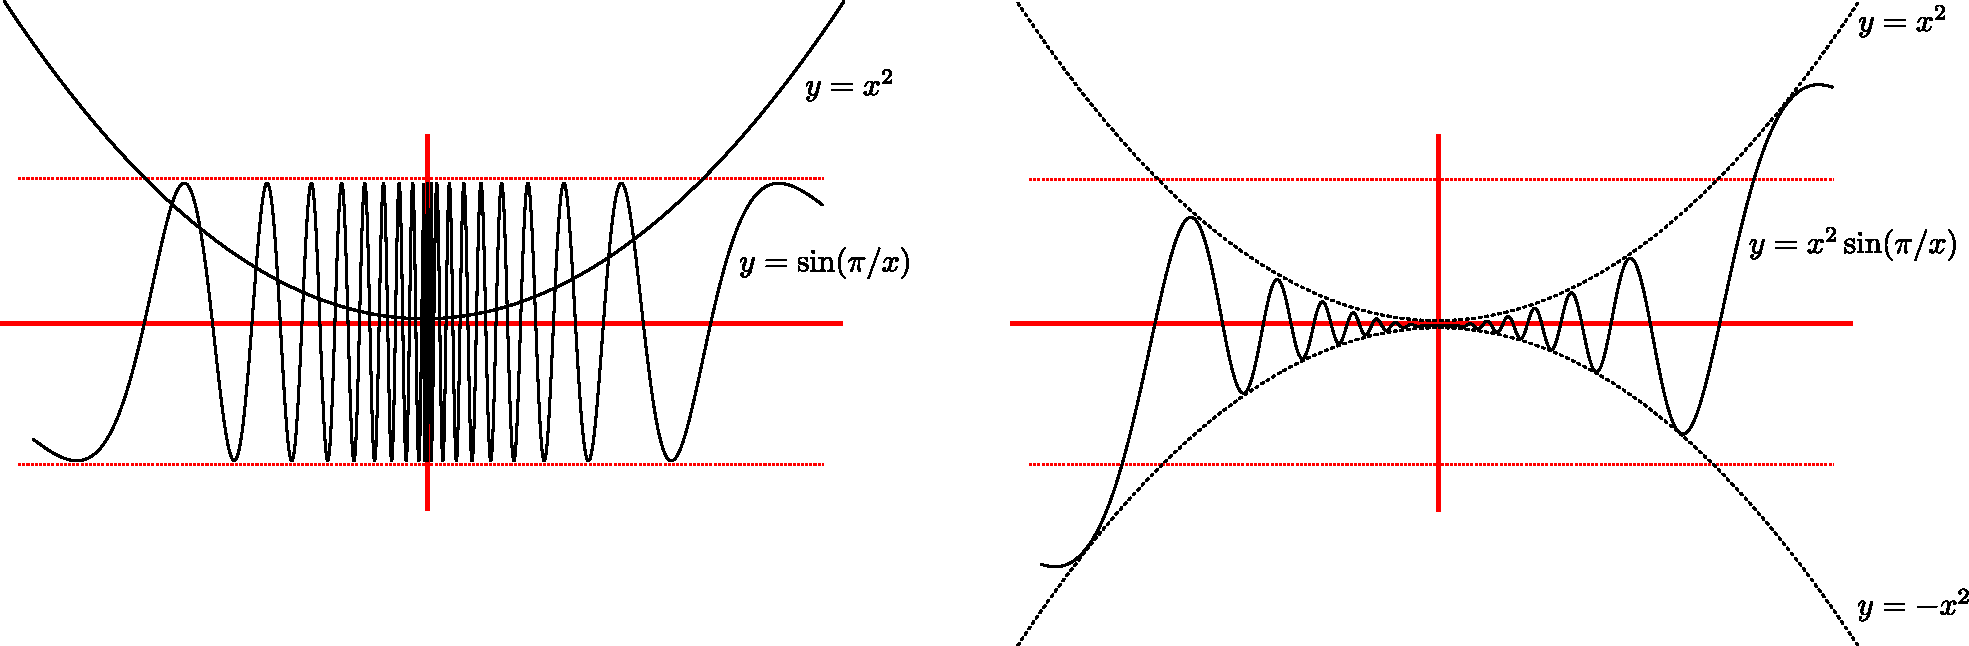
\includegraphics[width=\textwidth]{squeeze1}\\
\end{center}
\end{fig}
While $x^2$ is a very well behaved function and we know quite a lot about it,
the function $\sin(\pi/x)$ is quite ugly. One of the few things we can say
about it is the following
\begin{align*}
  -1 \leq \sin(\pi/x) \leq 1 && \text{provided $x \neq 0$}
\end{align*}
But if we multiply this expression by $x^2$ we get (because $x^2 \geq 0$)
\begin{align*}
  -x^2 \leq x^2\sin(\pi/x) \leq x^2 && \text{provided $x \neq 0$}
\end{align*}
and we have sketched the result in the figure above (on the right). So the
function we are interested in is \emph{squeezed} or \emph{sandwiched} between
the functions $x^2$ and $-x^2$.

If we focus in on the picture close to $x=0$ we see that $x$ approaches $0$,
the functions $x^2$ and $-x^2$ both approach $0$. Further, because
$x^2\sin(\pi/x)$ is sandwiched between them, it seems that it also approaches
$0$.

The following theorem tells us that this is indeed the case:
\begin{theorem}[Squeeze theorem (or sandwich theorem or pinch theorem)]
\label{thm squeeze}
  Let $a \in \mathbb{R}$ and let $f,g,h$ be three functions so that
  \begin{align*}
    f(x) \leq g(x) \leq h(x)
  \end{align*}
  for all $x$ in an interval around $a$, except possibly exactly at $x=a$. Then
if
  \begin{align*}
    \lim_{x \to a} f(x) &= \lim_{x \to a} h(x) = L
  \end{align*}
  then it is also the case that
  \begin{align*}
    \lim_{x \to a} g(x) &= L
  \end{align*}
\end{theorem}

Using the above theorem we can compute the limit we want and write it up nicely
\begin{eg}\label{eg_1_4_8}
  Compute the limit
\begin{align*}
  \lim_{x \to 0} x^2 \sin(\pi/x)
\end{align*}

  Since $-1 \leq \sin(\theta) \leq 1$ for all real numbers $\theta$, we have
\begin{align*}
  -1 \leq \sin(\pi /x ) \leq 1 && \text{for all $x \neq 0$}
\end{align*}
  Multiplying the above by $x^2$ we see that
\begin{align*}
  -x^2 \leq x^2 \sin(\pi /x ) \leq x^2 && \text{for all $x \neq 0$}
\end{align*}
  Since $\ds \lim_{x \to 0} x^2 = \lim_{x \to 0} (-x^2) = 0$ by the sandwich
(or squeeze or pinch) theorem we have
\begin{align*}
  \lim_{x \to 0} x^2 \sin(\pi/x) &= 0
\end{align*}
\end{eg}
Notice how we have used ``words''. We have remarked on this several times
already in the text, but we will keep mentioning it. It is okay to use words in
your answers to maths problems --- and you should do so! These let the reader
know what you are  doing and help you understand what you are doing.

Another sandwich theorem example
\begin{eg}\label{eg_1_4_9}
Let $f(x)$ be a function such that $1 \leq f(x) \leq x^2-2x+2$. What is
$\ds \lim_{x \to 1} f(x)$?

We are already supplied with an inequality, so it is likely that it is going to
help us. We should examine the limits of each side to see if they are the same:
\begin{align*}
  \lim_{x \to 1} 1 &= 1 \\
  \lim_{x \to 1} x^2-2x+2 &= 1-2+2 = 1
\end{align*}
So we see that the function $f(x)$ is trapped between two functions that both
approach $1$ as $x \to 1$. Hence by the sandwich / pinch / squeeze theorem, we
know that
\begin{align*}
  \lim_{x \to 1} f(x) & =1
\end{align*}
\end{eg}


To get some intuition as to why the squeeze theorem is true, consider when $x$ is very very close to $a$.
In particular, consider when $x$ is sufficiently close to $a$ that we know $h(x)$ is within $10^{-6}$ of $L$
and that $f(x)$ is also within $10^{-6}$ of $L$. That is
\begin{align*}
|h(x)-L| &<10^{-6}  & \text{and}&& |f(x)-L| &<10^{-6}.
\end{align*}
This means that
\begin{align*}
L-10^{-6} &< f(x) \leq h(x) < L+10^{-6}
\end{align*}
since we know that $f(x) \leq h(x)$.

But now by the hypothesis of the squeeze theorem we know that $f(x) \leq g(x) \leq h(x)$ and so we have
\begin{align*}
L-10^{-6} &< f(x) \leq g(x) \leq h(x) < L+10^{-6}
\end{align*}
And thus we know that
\begin{align}
L-10^{-6} &\leq g(x) \leq L+10^{-6}
\end{align}
That is $g(x)$ is also within $10^{-6}$ of $L$.

In this argument our choice of $10^{-6}$ was arbitrary, so we can really replace $10^{-6}$ with any small number we like.
Hence we know that we can force $g(x)$ as close to $L$ as we like, by bringing $x$ sufficiently close to $a$. We give
a more formal and rigorous version of this argument at the end of Section~\ref{sec proof arith lim}.

\section{Limits at Infinity}\label{sec_1_5}
Up until this point we have discussed what happens to a function as we move its input $x$
closer and closer to a particular point $a$. For a great many applications of
limits we need to understand what happens to a function when its input becomes
extremely large --- for example what happens to a population at a time far in
the future.

The definition of a limit at infinity has a similar flavour to the definition of limits at
finite points that we saw above, but the details are a little different. We also
need to distinguish between positive and negative infinity. As $x$ becomes
very large and positive it moves off towards $+\infty$ but when it becomes very
large and negative it moves off towards $-\infty$.


Again we give an informal definition; the full formal definition can be found
in (the optional) Section~\ref{sec lim inf formal} near the end of this chapter.
\begin{defn}[Limits at infinity --- informal]\label{def_1_5_1}
We write
\begin{align*}
\lim_{x \to \infty} f(x) &= L
\end{align*}
when the value of the function $f(x)$ gets closer and closer to $L$ as we make
$x$ larger and larger and positive.

Similarly we write
\begin{align*}
\lim_{x \to -\infty} f(x) &= L
\end{align*}
when the value of the function $f(x)$ gets closer and closer to $L$ as we make
$x$ larger and larger and negative.

\end{defn}

\begin{eg}\label{eg_1_5_1}
Consider the two functions depicted below
\begin{efig}
\begin{center}
 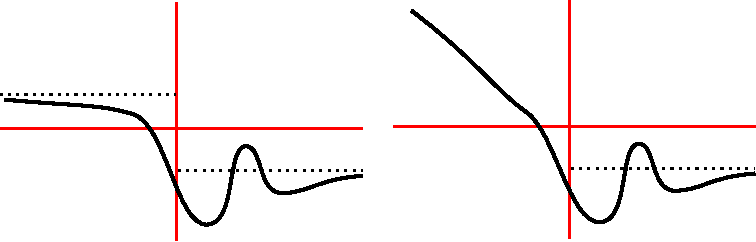
\includegraphics[height=4cm]{lim7}
\end{center}
\end{efig}
The dotted horizontal lines indicate the behaviour as $x$ becomes very large.
The function on the left has limits as $x \to \infty$ and as $x \to -\infty$
since  the function ``settles down'' to a particular value. On the other hand,
the function  on the right does not have a limit as $x \to -\infty$ since the
function just keeps getting bigger and bigger.
\end{eg}

Just as was the case for limits as $x \to a$ we will start with two very simple
building blocks and build other limits from those.
\begin{theorem}
\label{thm basic lim inf}
 Let $c \in \mathbb{R}$ then the following limits hold
\begin{align*}
  \lim_{x \to \infty} c &= c & \lim_{x \to -\infty} c &= c \\
  \lim_{x \to \infty} \frac{1}{x} &= 0 & \lim_{x \to -\infty} \frac{1}{x} &= 0
\end{align*}
\end{theorem}
Again, these limits interact nicely with standard arithmetic:
\begin{theorem}[Arithmetic of limits at infinity]\label{thm_1_5_1}
Let $f(x), g(x)$ be two functions for which the limits
 \begin{align*}
  \lim_{x \to \infty} f(x)&=F & \lim_{x \to \infty} g(x) &=G
\end{align*}
  exist. Then the following limits hold
\begin{align*}
  \lim_{x \to \infty} f(x) \pm g(x) &= F \pm G \\
  \lim_{x \to \infty} f(x) g(x) &= F  G \\
  \lim_{x \to \infty} \frac{f(x)}{ g(x) } &= \frac{F}{G} & \text{provided $G
\neq 0$}
\intertext{and for real numbers $p$}
  \lim_{x \to \infty} f(x)^p &= F^p & \text{provided $F^p$ and $f(x)^p$ are defined for all $x$}
\end{align*}
The analogous results hold for limits to $-\infty$.
\end{theorem}
Note that, as was the case in Theorem~\ref{thm lim powers}, we need a little extra care
with powers of functions. We must avoid taking square roots of negative numbers, or
indeed any even root of a negative number\footnote{To be more precise, there is no real
number $x$ so that $x^\text{even power}$ is a negative number. Hence we cannot take the
even-root of a negative number and express it as a real number. This is precisely
what complex numbers allow us to do, but alas there is not space in the course for us to
explore them.}.



Hence we have for all rational $r>0$
\begin{align*}
  \lim_{x \to \infty} \frac{1}{x^r} &= 0
\end{align*}
but we have to be careful with
\begin{align*}
  \lim_{x \to -\infty} \frac{1}{x^r} &= 0
\end{align*}
This is only true if the denominator of $r$ is not an even
number\footnote{where we write $r = \frac{p}{q}$ with $p,q$ integers with no
common factors. For example,  $r = \frac{6}{14}$ should be written as $r =
\frac{3}{7}$ when considering this rule.}.

For example
\begin{itemize}
 \item $\ds \lim_{x \to \infty} \frac{1}{x^{1/2}} = 0$, but $\ds \lim_{x \to
-\infty} \frac{1}{x^{1/2}}$ does not exist, because $x^{1/2}$ is not defined for
$x<0$.
\item On the other hand, $x^{4/3}$ is defined for negative values of $x$
and $\ds \lim_{x \to -\infty} \frac{1}{x^{4/3}} = 0$.
\end{itemize}

Our first application of limits at infinity will be to examine the behaviour of
a rational function for very large $x$. To do this we use a ``trick''.
\begin{eg}\label{eg_1_5_2}
Compute the following limit:
\begin{align*}
\lim_{x \to \infty} \frac{x^2-3x+4}{3x^2+8x+1}
\end{align*}
As $x$ becomes very  large, it is the $x^2$ term that will dominate in both the
numerator and denominator and the other bits become irrelevant. That is,
for very large $x$, $x^2$ is much much larger than $x$ or any constant. So we
pull out these dominant parts
\begin{align*}
  \frac{x^2-3x+4}{3x^2+8x+1}
  &= \frac{x^2 \left(1-\frac{3}{x}+\frac{4}{x^2}\right)}
  {x^2 \left(3+\frac{8}{x}+\frac{1}{x^2} \right)}\\
  &= \frac{1-\frac{3}{x}+\frac{4}{x^2}}
  {3+\frac{8}{x}+\frac{1}{x^2}} & \text{ remove the common factors}
\end{align*}
\begin{align*}
  \lim_{x \to \infty} \frac{x^2-3x+4}{3x^2+8x+1}
  &= \lim_{x \to \infty} \frac{1-\frac{3}{x}+\frac{4}{x^2}}
  {3+\frac{8}{x}+\frac{1}{x^2}}\\
  &= \frac{\ds \lim_{x \to \infty}\left(1-\frac{3}{x}+\frac{4}{x^2}\right)}
{\ds \lim_{x \to \infty}\left(3+\frac{8}{x}+\frac{1}{x^2} \right)}
& \text{arithmetic of limits} \\
  &= \frac{\ds \lim_{x \to \infty} 1
  - \lim_{x \to \infty} \frac{3}{x} + \lim_{x \to \infty} \frac{4}{x^2}}
{\ds \lim_{x \to \infty} 3
 + \lim_{x \to \infty} \frac{8}{x}+ \lim_{x \to \infty} \frac{1}{x^2} }
& \text{more arithmetic of limits} \\
  &= \frac{1+0+0}{3+0+0}  = \frac{1}{3}
\end{align*}
\end{eg}

The following one gets a little harder
\begin{eg}\label{eg lim tricky}
 Find the limit as $x \to \infty$ of $\frac{\sqrt{4x^2+1}}{5x-1}$

We use the same trick --- try to work out what is the biggest term in the
numerator and denominator and pull it to one side.
\begin{itemize}
 \item The denominator is dominated by $5x$.
 \item The biggest contribution to the numerator comes from the $4x^2$ inside
the square-root. When we pull $x^2$ outside the square-root it becomes $x$,
so the numerator is dominated by $x \cdot \sqrt{4} = 2x$
 \item To see this more explicitly rewrite the numerator
\begin{align*}
  \sqrt{4x^2+1} &= \sqrt{x^2 (4+1/x^2)} = \sqrt{x^2} \sqrt{4+1/x^2} =
x\sqrt{4+1/x^2}.
\end{align*}
\item Thus the limit as $x \to \infty$ is
\begin{align*}
 \lim_{x \to \infty} \frac{\sqrt{4x^2+1}}{5x-1}
 &= \lim_{x \to \infty} \frac{x \sqrt{4+1/x^2}}{x(5-1/x)}\\
 &= \lim_{x \to \infty} \frac{\sqrt{4+1/x^2}}{5-1/x} \\
 & = \frac{2}{5}
\end{align*}
\end{itemize}
\end{eg}

Now let us also think about the limit of the same function,
$\frac{\sqrt{4x^2+1}}{5x-1}$, as $x \rightarrow -\infty$. There is something
subtle going on because of the square-root. First consider the
function\footnote{Just to change things up let's use $t$ and $h(t)$ instead of
the ubiquitous $x$ and $f(x)$.}
\begin{align*}
  h(t) &= \sqrt{t^2}
\end{align*}
Evaluating this at $t=7$ gives
\begin{align*}
  h(7) &= \sqrt{ 7^2 } = \sqrt{49} = 7
\end{align*}
We'll get much the same thing for any $t \geq 0$. For any $t \ge 0$, $h(t)=\sqrt{t^2}$
returns exactly $t$. However now consider the function at $t=-3$
\begin{align*}
  h(-3) &= \sqrt{ (-3)^2 } = \sqrt{9} = 3 = - (-3)
\end{align*}
that is the function is returning $-1$ times the input.

This is because when we defined $\sqrt{\text{ }}$, we defined it to be the
\emph{positive} square-root. i.e. the function $\sqrt{t}$ can never return a
negative number. So being more careful
\begin{align*}
  h(t) &= \sqrt{t^2} = | t |
\end{align*}
Where the $|t|$ is the absolute value of $t$. You are perhaps used to thinking
of absolute value as ``remove the minus sign'', but this is not quite correct.
Let's sketch the function
\begin{fig}
\begin{center}
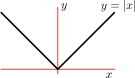
\includegraphics[height=3cm]{abs}
\end{center}
\end{fig}
It is a piecewise function defined by
\begin{align*}
  |x| &= \begin{cases}
          x & x \geq 0\\
	  -x & x < 0
         \end{cases}
\end{align*}
Hence our function $h(t)$ is really
\begin{align*}
  h(t) &= \sqrt{t^2} =
	  \begin{cases}
          t & t \geq 0\\
	  -t & t < 0
         \end{cases}
\end{align*}
So that when we evaluate $h(-7)$ it is
\begin{align*}
  h(-7) &= \sqrt{ (-7)^2 } = \sqrt{49} = 7 = -(-7)
\end{align*}
We are now ready to examine the limit as $x \to -\infty$ in our previous
example. Mostly it is copy and paste from above.
\begin{eg}\label{eg lim tricky part2}
 Find the limit as $x \to -\infty$ of $\frac{\sqrt{4x^2+1}}{5x-1}$

We use the same trick --- try to work out what is the biggest term in the
numerator and denominator and pull it to one side. Since we are taking the
limit as $x \to -\infty$ we should think of $x$ as a large negative number.
\begin{itemize}
 \item The denominator is dominated by $5x$.
 \item The biggest contribution to the numerator comes from the $4x^2$ inside
the square-root. When we pull the $x^2$ outside a square-root it becomes $|x| =
-x$ (since we are taking the limit as $x \to -\infty$), so the numerator is
dominated by $-x\cdot\sqrt{4} = -2x$
 \item To see this more explicitly rewrite the numerator
\begin{align*}
  \sqrt{4x^2+1} &= \sqrt{x^2 (4+1/x^2)}  = \sqrt{x^2} \sqrt{4+1/x^2} \\
  &= |x|\sqrt{4+1/x^2} & \text{ and since $x<0$ we have} \\
  & = -x\sqrt{4+1/x^2}
\end{align*}
\item Thus the limit as $x \to -\infty$ is
\begin{align*}
 \lim_{x \to -\infty} \frac{\sqrt{4x^2+1}}{5x-1}
 &= \lim_{x \to -\infty} \frac{-x \sqrt{4+1/x^2}}{x(5-1/x)}\\
 &= \lim_{x \to -\infty} \frac{-\sqrt{4+1/x^2}}{5-1/x} \\
 & = -\frac{2}{5}
\end{align*}
\end{itemize}
\end{eg}
So the limit as $x \to -\infty$ is almost the same but we gain a minus sign.
This \textbf{is definitely not} the case in general --- you have to think about each
example separately.

Here is a sketch of the function in question.
\begin{fig}
\begin{center}
 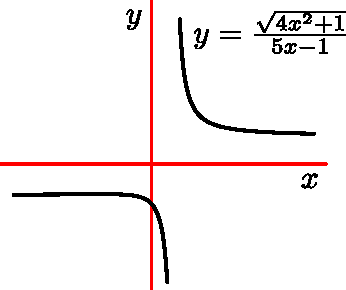
\includegraphics[height=4cm]{neg_inf_lim}
\end{center}
\end{fig}


\begin{eg}\label{eg_1_5_3}
Compute the following limit:
\begin{align*}
  \lim_{x \to \infty} \left( x^{7/5}-x \right)
\end{align*}
In this case we cannot use the arithmetic of limits to write this as
\begin{align*}
  \lim_{x \to \infty} \left( x^{7/5}-x \right)
  &= \left( \lim_{x \to \infty} x^{7/5}\right)
  - \left( \lim_{x \to \infty} x \right) \\
  &= \infty -\infty
\end{align*}
because the limits do not exist. We can only use the limit laws when the limits
exist. So we should go back and think some more.

When $x$ is very large, $x^{7/5} = x\cdot x^{2/5}$ will be much larger than $x$, so the
$x^{7/5}$ term will dominate the $x$ term. So factor out $x^{7/5}$ and rewrite it as
\begin{align*}
  x^{7/5}-x &= x^{7/5} \left(1 - \frac{1}{x^{2/5}} \right)
\end{align*}
Consider what happens to each of the factors as $x \to \infty$
\begin{itemize}
 \item For large $x$, $x^{7/5}>x$ (this is actually true for any $x>1$).
In the limit as $x \to +\infty$, $x$ becomes arbitrarily large and
positive, and $x^{7/5}$ must be bigger still, so it follows that
\begin{align*}
  \lim_{x \to \infty} x^{7/5} &= + \infty.
\end{align*}
 \item On the other hand, $(1-x^{-2/5})$ becomes closer and closer to $1$ ---
we can use the arithmetic of limits to write this as
\begin{align*}
  \lim_{x \to \infty} (1-x^{-2/5}) &= \lim_{x \to \infty} 1 - \lim_{x \to
\infty} x^{-2/5} = 1-0 = 1
\end{align*}
\end{itemize}
So the product of these two factors will be come larger and larger (and
positive) as $x$ moves off to infinity. Hence we have
\begin{align*}
  \lim_{x \to \infty} x^{7/5} \left(1 - 1/x^{2/5} \right) &= + \infty
\end{align*}
\end{eg}
But remember $+\infty$ and $-\infty$ are not numbers; the last equation in the example is
shorthand for ``the function becomes arbitrarily large''.

In the previous section we saw that finite limits and arithmetic interact very nicely
(see Theorems~\ref{thm arith lim} and~\ref{thm lim powers}). This enabled us to compute
the limits of more complicated function in terms of simpler ones. When limits of
functions go to plus or minus infinity we are quite a bit more restricted in what we can
deduce. The next theorem states some results concerning the sum, difference, ratio and
product of infinite limits --- unfortunately in many cases we cannot make general
statements and the results will depend on the details of the problem at hand.

\begin{theorem}[Arithmetic of infinite limits]
\label{thm arith inf lim}
 Let $a,c,H \in \mathbb{R}$ and let $f,g,h$ be functions defined in
an interval around $a$ (but they need not be defined at $x=a$), so that
\begin{align*}
  \lim_{x \to a} f(x) &= +\infty &
  \lim_{x \to a} g(x) &= +\infty &
  \lim_{x \to a} h(x) &= H
\end{align*}
\begin{itemize}
 \item $\ds \lim_{x \to a} ( f(x) + g(x) ) = +\infty$
 \item $\ds \lim_{x \to a} ( f(x) + h(x) ) = +\infty$
 \item $\ds \lim_{x \to a} ( f(x) - g(x) )$ undetermined
 \item $\ds \lim_{x \to a} ( f(x) - h(x) ) = +\infty$
 \item $\ds \lim_{x \to a} c f(x) =
\begin{cases}
 +\infty & c>0 \\
0 & c=0 \\
-\infty & c<0
\end{cases}
$
\item $\ds \lim_{x \to a} ( f(x) \cdot g(x) ) = +\infty$.
\item $\ds \lim_{x \to a} f(x) h(x) =
\begin{cases}
 +\infty & H>0 \\
-\infty & H<0\\
\text{undetermined} & H=0
\end{cases}
$
\item $\ds \lim_{x \to a} \frac{f(x)}{g(x)}$ undetermined
\item $\ds \lim_{x \to a} \frac{f(x)}{h(x)} =
\begin{cases}
+\infty & H>0 \\
-\infty & H<0\\
\text{undetermined} & H=0
\end{cases}$

%\end{itemize}
%\end{theorem}
%
%\addtocounter{theorem}{-1}
%\begin{theorem}[continued]
%\begin{itemize}

\item $\ds \lim_{x \to a} \frac{h(x)}{f(x)} = 0$

\item $\ds \lim_{x \to a} f(x)^p =
\begin{cases}
+\infty & p>0 \\
0 & p<0\\
1 & p=0
\end{cases}$
\end{itemize}
\end{theorem}
Note that by ``undetermined'' we mean that the limit may or may not exist, but
cannot be determined from the information given in the theorem. See
Example~\ref{eg lim rat} for an example of what we mean by
``undetermined''. Additionally consider the following example.
\begin{eg}\label{eg_1_5_4}
Consider the following 3 functions:
\begin{align*}
f(x)&=x^{-2} & g(x)&=2x^{-2} &h(x)&=x^{-2}-1. \\
\intertext{Their limits as $x \to 0$ are:}
\lim_{x\to0} f(x) &= +\infty &
\lim_{x\to0} g(x) &= +\infty &
\lim_{x\to0} h(x) &= +\infty.
\end{align*}
Say we want to compute the limit of the difference of two of the above functions as $x
\to 0$. Then the previous theorem cannot help us. This is not because it is too weak,
rather it is because the difference of two infinite limits can be, either plus infinity,
minus infinity or some finite number depending on the details of the problem. For example,
\begin{align*}
  \lim_{x\to0} \left( f(x)-g(x) \right) &= \lim_{x\to0} -x^{-2} = -\infty \\
  \lim_{x\to0} \left( f(x)-h(x) \right) &= \lim_{x\to0} 1 = 1 \\
  \lim_{x\to0} \left( g(x)-h(x) \right) &= \lim_{x\to0} x^{-2}+1 = +\infty
\end{align*}


\end{eg}






\section{Continuity}\label{sec_1_6}
We have seen that computing the limits some functions --- polynomials and
rational functions --- is very easy because
\begin{align*}
  \lim_{x \to a} f(x) &= f(a).
\end{align*}
That is, the limit as $x$ approaches $a$ is just $f(a)$. Roughly speaking,
the reason we can compute the limit this way is that these functions do not
have any abrupt jumps near $a$.

Many other functions have this property, $\sin(x)$ for example. A function
with this property is called ``continuous'' and there is a precise mathematical definition
for it. If you do not recall interval notation, then now is a good time to take a quick
look back at Definition~\ref{def intervals}.
\begin{defn}\label{def_1_6_1}
A function $f(x)$ is continuous at $a$ if
\begin{align*}
	\lim_{x \to a} f(x) &= f(a).
\end{align*}
If a function is not continuous at $a$ then it is said to be discontinuous
at~$a$.

When we write that $f$ is continuous without specifying a point, then typically
this means that $f$ is continuous at $a$ for all $a \in \mathbb{R}$.

When we write that $f(x)$ is continuous on the open interval $(a,b)$ then the function is
continuous at every point $c$ satisfying $a<c<b$.
\end{defn}

So if a function is continuous at $x=a$ we immediately know that
\begin{itemize}
 \item $f(a)$ exists
 \item $\ds \lim_{x \to a^-}$ exists and is equal to $f(a)$, and
 \item $\ds \lim_{x \to a^+}$ exists and is equal to $f(a)$.
\end{itemize}

\subsection*{Quick Aside --- One-sided Continuity}
Notice in the above definition of continuity on an interval $(a,b)$ we have carefully
avoided saying anything about whether or not the function is continuous at the endpoints
of the interval --- i.e. is $f(x)$ continuous at $x=a$ or $x=b$. This is because talking
of
continuity at the endpoints of an interval can be a little delicate.

In many situations we will be given a function $f(x)$ defined on a closed interval
$[a,b]$. For example, we might have:
\begin{align*}
  f(x) &= \frac{x+1}{x+2} & \text{for $x \in [0,1]$}.
\end{align*}
For any $0 \leq x \leq 1$ we know the value of $f(x)$. However for $x<0$ or $x>1$ we
know nothing about the function --- indeed it has not been defined.

So now, consider what it means for $f(x)$ to be continuous at $x=0$. We need to have
\begin{align*}
  \lim_{x\to 0} f(x) &= f(0),
\end{align*}
however this implies that the one-sided limits
\begin{align*}
  \lim_{x\to 0^+} f(x) &= f(0) & \text{and}&& \lim_{x\to 0^-} f(x) &= f(0)
\end{align*}
Now the first of these one-sided limits involves examining the behaviour of $f(x)$ for
$x>0$. Since this involves looking at points for which $f(x)$ is defined, this is
something we can do. On the other hand the second one-sided limit requires us to
understand the behaviour of $f(x)$ for $x<0$. This we cannot do because the function
hasn't been defined for $x<0$.

One way around this problem is to generalise the idea of continuity to one-sided
continuity, just as we generalised limits to get one-sided limits.
\begin{defn}\label{def_1_6_2}
  A function $f(x)$ is continuous from the right at $a$ if
  \begin{align*}
    \lim_{x\to a^+} f(x) &= f(a).
  \end{align*}
  Similarly a function $f(x)$ is continuous from the left at $a$ if
  \begin{align*}
    \lim_{x\to a^-} f(x) &= f(a)
  \end{align*}
\end{defn}

Using the definition of one-sided continuity we can now define what it means for a
function to be continuous on a closed interval.
\begin{defn}\label{def_1_6_3}
 A function $f(x)$ is continuous on the closed interval $[a,b]$ when
\begin{itemize}
 \item $f(x)$ is continuous on $(a,b)$,
 \item $f(x)$ is continuous from the right at $a$, and
 \item $f(x)$ is continuous from the left at $b$.
\end{itemize}
Note that the last two condition are equivalent to
\begin{align*}
   \lim_{x\to a^+} f(x) &= f(a) & \text{ and }&&
  \lim_{x\to b^-} f(x) &= f(b).
\end{align*}
\end{defn}

\subsection*{Back to the Main Text}


We already know from our work above that polynomials are continuous, and that
rational functions are continuous at all points in their domains --- i.e. where
their denominators are non-zero. As we did for
limits, we will see that continuity interacts ``nicely'' with arithmetic. This
will allow us to construct complicated continuous functions from simpler
continuous building blocks (like polynomials).

But first, a few examples\dots
\begin{eg}\label{eg_1_6_1}
Consider the functions drawn below
\begin{efig}
\begin{center}
 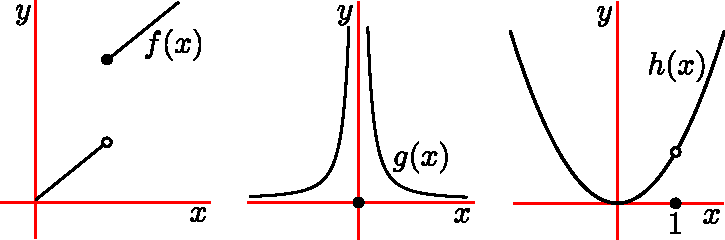
\includegraphics[height=4cm]{lim6}\\
\end{center}
\end{efig}
These are
\begin{align*}
f(x) &= \begin{cases} x&x<1 \\ x+2 & x\geq 1 \end{cases}
&
g(x) &= \begin{cases} 1/x^2& x\neq0 \\ 0 & x=0\end{cases}
&
h(x) &= \begin{cases}\frac{x^3-x^2}{x-1} & x\neq 1\\ 0 & x=1 \end{cases}
\end{align*}
Determine where they are continuous and discontinuous:
\begin{itemize}
\item When $x<1$ then $f(x)$ is a straight line (and so a polynomial) and so it is
continuous at every point $x<1$. Similarly when $x>1$ the function is a
straight line and so it is continuous at every point $x>1$. The only point which
might be a discontinuity is at $x=1$. We see that the one sided limits are
different. Hence the limit at $x=1$ does not exist and so the function is
discontinuous at $x=1$.

But note that that $f(x)$ is continuous from one side --- which?

\item The middle case is much like the previous one. When $x \neq 0$ the $g(x)$
is a rational function and so is continuous everywhere on its domain (which is
all reals except $x=0$). Thus the only point where $g(x)$ might be discontinuous is at
$x=0$. We see that neither of the one-sided limits exist at $x=0$, so the limit
does not exist at $x=0$. Hence the function is discontinuous at $x=0$.

\item We have seen the function $h(x)$ before. By the same reasoning as
above, we know it is continuous except at $x=1$ which we must check separately.

By definition of $h(x)$, $h(1) = 0$. We must compare this to the limit as $x
\to 1$. We did this before.
\begin{align*}
	\frac{x^3-x^2}{x-1} &= \frac{x^2(x-1)}{x-1} = x^2
\end{align*}
So $\lim_{x \to 1} \frac{x^3-x^2}{x-1} = \lim_{x \to 1} x^2 
= 1\neq h(1)$. Hence $h$
is discontinuous at $x=1$.
\end{itemize}
\end{eg}

This example illustrates different sorts of discontinuities:
\begin{itemize}
\item The function $f(x)$ has a ``jump discontinuity'' because the function
``jumps'' from one finite value on the left to another value on the right.
\item The second function, $g(x)$, has an ``infinite discontinuity'' since
$\lim f(x) =+\infty$.
\item The third function, $h(x)$, has a ``removable discontinuity'' because we
could make the function continuous at that point by redefining the function at
that point. i.e. setting $h(1)=1$. That is
\begin{align*}
  \text{new function }h(x) &= \begin{cases}
    \frac{x^3-x^2}{x-1} & x\neq 1\\
    1 & x=1
    \end{cases}
\end{align*}
\end{itemize}


Showing a function is continuous can be a pain, but just as the limit laws help
us compute complicated limits in terms of simpler limits, we can use them to
show that complicated functions are continuous by breaking them into simpler
pieces.
\begin{theorem}[Arithmetic of continuity]\label{thm arith cont}
  Let $a,c \in \mathbb{R}$ and let $f(x)$ and $g(x)$ be functions that are
continuous at $a$. Then the following functions are also continuous at $x=a$:
\begin{itemize}
 \item $f(x) + g(x)$ and $f(x) - g(x)$,
 \item $c f(x)$ and $f(x) g(x)$, and
 \item $\frac{f(x)}{g(x)}$ provided $g(a) \neq 0$.
\end{itemize}
\end{theorem}

Above we stated that polynomials and rational functions are
continuous (being careful about domains of rational functions ---
we must avoid the denominators being zero) without making it a formal
statement. This is easily fixed\dots

\begin{lemma}\label{lem_1_6_1}
 Let $c \in \mathbb{R}$. The functions
  \begin{align*}
  f(x) &= x & g(x) &= c
  \end{align*}
  are continuous everywhere on the real line
\end{lemma}
This isn't quite the result we wanted (that's a couple of lines below) but it
is a small result that we can combine with the arithmetic of limits to get the
result we want. Such small helpful results are called ``lemmas'' and they will
arise more as we go along.

Now since we can obtain any polynomial and any rational function by carefully
adding, subtracting, multiplying and dividing the functions $f(x)=x$ and
$g(x)=c$, the above lemma combines with the ``arithmetic of continuity''
theorem to give us the result we want:
%
\begin{theorem}[Continuity of polynomials and rational functions]
\label{thm_1_6_1}
Every polynomial is continuous everywhere. Similarly every rational
function is continuous except where its denominator is zero (i.e. on all its
domain).
\end{theorem}

With some more work this result can be extended to wider families of functions:
\begin{theorem}\label{thm_1_6_2}
The following functions are continuous everywhere in their domains
\begin{itemize}
\item polynomials, rational functions
\item roots and powers
\item trig functions and their inverses
\item exponential and the logarithm
\end{itemize}
\end{theorem}
We haven't encountered inverse trigonometric functions, nor exponential
functions or logarithms, but we will see them in the next chapter. For the
moment, just file the information away.


Using a combination of the above results you can show that many complicated
functions are continuous except at a few points (usually where a denominator is
equal to zero).
\begin{eg}\label{eg_1_6_2}
Where is the function $f(x) = \frac{\sin(x)}{2+\cos(x)}$ continuous?

We just break things down into pieces and then put them back together keeping
track of where things might go wrong.
 \begin{itemize}
  \item The function is a ratio of two pieces --- so check if the numerator is
continuous, the denominator is continuous, and if the denominator might be zero.
  \item The numerator is $\sin(x)$ which is ``continuous on its domain''
according to one of the above theorems. Its domain is all real
numbers\footnote{Remember that $\sin$ and $\cos$ are defined on all real numbers, so
$\tan(x) = \sin(x)/\cos(x)$ is continuous everywhere except where $\cos(x)=0$. This
happens when $x = \frac{\pi}{2}+n\pi$ for any integer $n$. If you cannot remember where
$\tan(x)$ ``blows up'' or $\sin(x)=0$ or $\cos(x)=0$ then you should definitely revise
trigonometric functions. Come to think of it --- just revise them anyway.}, so it is
continuous everywhere. No problems here.

 \item The denominator is the sum of $2$ and $\cos(x)$. Since $2$ is a constant
it is continuous everywhere. Similarly (we just checked things for the
previous point) we know that $\cos(x)$ is continuous everywhere. Hence the
denominator is continuous.

 \item So we just need to check if the denominator is zero. One of the facts
that we should know\footnote{If you do not know this fact then you should
revise trigonometric functions. See the previous footnote.} is that
\begin{align*}
  -1 \leq \cos(x) \leq 1
\intertext{and so by adding 2 we get}
  1 \leq 2+\cos(x) \leq 3
\end{align*}
Thus no matter what value of $x$, $2+\cos(x) \geq 1$ and so cannot be zero.

 \item So the numerator is continuous, the denominator is continuous and
nowhere zero, so the function is continuous everywhere.
 \end{itemize}

If the function were changed to $\ds \frac{\sin(x)}{x^2-5x+6}$ much of the same
reasoning can be used. Being a little terse we could answer with:
  \begin{itemize}
   \item Numerator and denominator are continuous.
   \item Since $x^2-5x+6=(x-2)(x-3)$ the denominator is zero when $x=2,3$.
   \item So the function is continuous everywhere except possibly
at $x=2,3$. In order to verify that the function really is discontinuous at
those points, it suffices to verify that the numerator is non-zero at $x=2,3$.
Indeed we know that $\sin(x)$ is zero only when $x = n\pi$ (for any integer
$n$). Hence $\sin(2),\sin(3) \neq 0$. Thus the numerator is non-zero, while the
denominator is zero and hence $x=2,3$ really are points of discontinuity.
\end{itemize}
Note that this example raises a subtle point about checking continuity when
numerator and denominator are \emph{simultaneously} zero. There are quite a
few possible outcomes in this case and we need more sophisticated tools to
adequately analyse the behaviour of functions near such points. We will return
to this question later in the text after we have developed Taylor expansions (see
Section~\ref{sec:DIFFTaylor}).
\end{eg}

So we know what happens when we add subtract multiply and divide, what about
when we compose functions? Well - limits and compositions work nicely when
things are continuous.
\begin{theorem}[Compositions and continuity]\label{thm comp cont}
  If $f$ is continuous at $b$ and $\ds \lim_{x \to a} g(x) = b$ then
$\ds \lim_{x\to a} f(g(x)) = f(b)$. I.e.
  \begin{align*}
   \lim_{x \to a} f\left( g(x) \right) &= f\left( \lim_{x \to a} g(x) \right)
  \end{align*}
Hence if $g$ is continuous at $a$ and $f$ is continuous at $g(a)$ then the
composite function $(f \circ g)(x) = f(g(x))$ is continuous at $a$.
\end{theorem}
So when we compose two continuous functions we get a new continuous function.

We can put this to use
\begin{eg}\label{eg_1_6_3}
Where are the following functions continuous?
\begin{align*}
  f(x) &= \sin\left( x^2 +\cos(x) \right) \\
  g(x) &= \sqrt{\sin(x)}
\end{align*}
Our first step should be to break the functions down into pieces and study
them. When we put them back together we should be careful of dividing by zero,
or falling outside the domain.
\begin{itemize}
 \item The function $f(x)$ is the composition of $\sin(x)$ with $x^2+\cos(x)$.
 \item These pieces, $\sin(x), x^2, \cos(x)$ are continuous everywhere.
 \item So the sum $x^2+\cos(x)$ is continuous everywhere
 \item And hence the composition of $\sin(x)$ and $x^2+\cos(x)$ is continuous
everywhere.
\end{itemize}
The second function is a little trickier.
\begin{itemize}
 \item The function $g(x)$ is the composition of $\sqrt{x}$ with $\sin(x)$.
 \item $\sqrt{x}$ is continuous on its domain $x \geq 0$.
 \item $\sin(x)$ is continuous everywhere, but it is negative in many places.
 \item In order for $g(x)$ to be defined and continuous we must restrict $x$ so that
$\sin(x) \geq 0$.
 \item Recall the graph of $\sin(x)$:
\begin{efig}
\begin{center}
 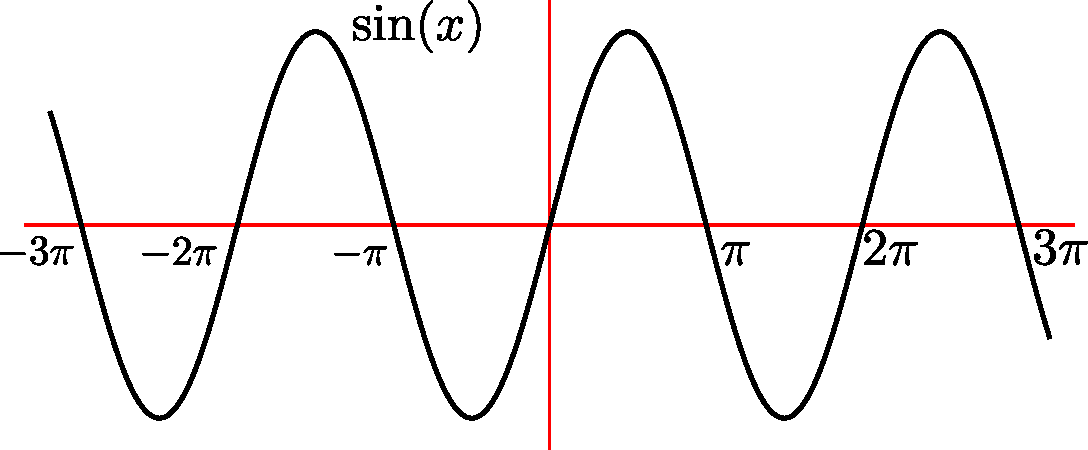
\includegraphics[height=35mm]{sinx}
\end{center}
\end{efig}
 Hence $\sin(x)\geq 0$ when $x\in[0,\pi]$ or $x\in [2\pi,3\pi]$ or $x\in[-2\pi,-\pi]$
or\dots. To be more precise $\sin(x)$ is positive when $x \in [2n\pi,(2n+1)\pi]$ for any
integer $n$.
\item Hence $g(x)$ is continuous when $x \in [2n\pi,(2n+1)\pi]$ for any
integer $n$.
\end{itemize}

% \begin{itemize}
%  \item $\log(\sin(x)^2)$ ---
%  \begin{itemize}
%   \item $\log(x)$ is continuous for all $x \geq 0$.
%   \item $\sin(x)^2 \geq 0$ for all $x$.
%   \item $\sin(x)^2$ is zero when $x=n \pi$.
%  \end{itemize}
%  is continuous except when $x=n \pi$, $n=0,\pm1,\pm2,\pm3, \dots$.
% \end{itemize}
\end{eg}

Continuous functions are very nice (mathematically speaking). Functions
from the ``real world'' tend to be continuous (though not always). The key
aspect that  makes them nice is the fact that they don't jump about.

The absence of such jumps leads to the following theorem which, while it can be
quite confusing on first glance, actually says something very natural ---
obvious even. It says, roughly speaking, that, as you draw the graph $y=f(x)$ starting at
$x=a$ and ending at $x=b$, $y$ changes continuously from $y=f(a)$ to $y=f(b)$, with no
jumps, and consequently $y$ must take every value between $f(a)$ and $f(b)$ at least once.
We'll start by just giving the precise statement and then we'll explain it in detail.
\begin{theorem}[Intermediate value theorem (IVT)]
\label{thm ivt}
Let $a<b$ and let $f$ be a function that is continuous at all points $a\leq x
\leq b$. If $Y$ is any number between $f(a)$ and $f(b)$ then there exists some
number $c \in [a,b]$ so that $f(c) = Y$.
\end{theorem}
Like the $\epsilon-\delta$ definition of limits\footnote{The interested student is
invited to take a look at the optional Section~\ref{sec opt formal limit}}, we should
break this
theorem down into pieces. Before we do that, keep the following pictures in mind.
\begin{fig}
\begin{center}
 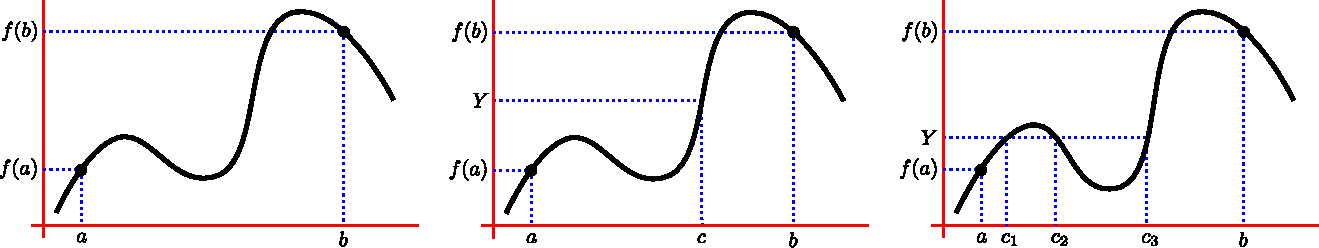
\includegraphics[width=\textwidth]{IVT}
\end{center}
\end{fig}
Now the break-down
\begin{itemize}
 \item \textbf{Let $a<b$ and let $f$ be a function that is continuous at all
points $a\leq x \leq b$.} --- This is setting the scene. We have $a,b$ with
$a<b$ (we can safely assume these to be real numbers). Our function must
be continuous at all points between $a$ and $b$.

\item \textbf{if $Y$ is any number between $f(a)$ and $f(b)$} --- Now we need
another number $Y$ and the only restriction on it is that it lies between
$f(a)$ and $f(b)$. That is, if $f(a)\leq f(b)$ then $f(a) \leq Y \leq f(b)$. Or
if $f(a) \geq f(b)$ then $f(a) \geq Y \geq f(b)$. So notice that $Y$ could be
equal to $f(a)$ or $f(b)$ --- if we wanted to avoid that possibility, then we
would normally explicitly say $Y \neq f(a), f(b)$ or we would write that $Y$
is \emph{strictly} between $f(a)$ and $f(b)$.

\item \textbf{there exists some number $c \in [a,b]$ so that $f(c) = Y$} --- so
if we satisfy all of the above conditions, then there has to be some real
number $c$ lying between $a$ and $b$ so that when we evaluate $f(c)$ it is $Y$.
\end{itemize}
So that breaks down the proof statement by statement, but what does it actually
mean?
\begin{itemize}
 \item Draw any continuous function you like between $a$ and $b$ --- it must be
continuous.
 \item The function takes the value $f(a)$ at $x=a$ and $f(b)$ at $x=b$ --- see
the left-hand figure above.
 \item Now we can pick any $Y$ that lies between $f(a)$ and $f(b)$ --- see the
middle figure above. The IVT\footnote{Often with big important useful theorems
like this one, writing out the full name again and again becomes tedious, so we
abbreviate it. Such abbreviations are okay provided the reader knows this is
what you are doing, so the first time you use an abbreviation you should let
the reader know. Much like we are doing here in this footnote: ``IVT'' stands for ``intermediate value theorem'', which is Theorem~\ref{thm ivt}.} tells us that
there must be some $x$-value that when plugged into the function gives us $Y$.
That is, there is some $c$ between $a$ and $b$ so that $f(c) = Y$. We can also interpret
this graphically; the IVT tells us that the horizontal straight line $y=Y$ must intersect
the graph $y=f(x)$ at some point $(c,Y)$ with $a\le c\le b$.

\item Notice that the IVT does not tell us how many such $c$-values there are,
just that there is at least one of them. See the right-hand figure above. For
that particular choice of $Y$ there are three different $c$ values so that
$f(c_1) = f(c_2) = f(c_3) = Y$.
\end{itemize}
This theorem says that if $f(x)$ is a continuous function on all of the
interval $a \leq x \leq b$ then as $x$ moves from $a$ to $b$, $f(x)$ takes every
value between $f(a)$ and $f(b)$ at least once. To put this slightly
differently, if $f$ were to avoid a value between $f(a)$ and $f(b)$ then $f$
cannot be continuous on $[a,b]$.


It is not hard to convince yourself that the continuity of $f$ is crucial to
the IVT. Without it one can quickly construct examples of functions that
contradict the theorem. See the figure below for a few non-continuous examples:
\begin{fig}
\begin{center}
 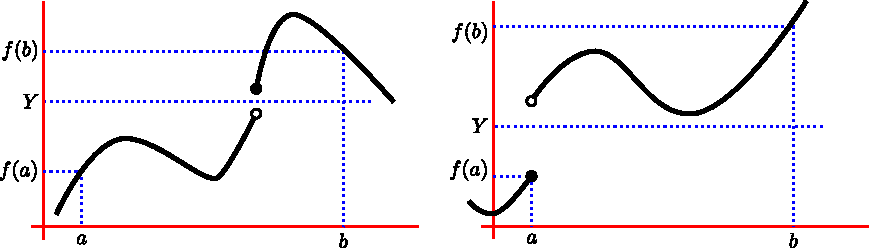
\includegraphics[height=4cm]{IVT2}
\end{center}
\end{fig}
In the left-hand example we see that a discontinuous function can ``jump'' over
the $Y$-value we have chosen, so there is no $x$-value that makes $f(x)=Y$. The
right-hand example demonstrates why we need to be be careful with the ends of
the interval. In particular, a function must be continuous over the whole
interval $[a,b]$ \emph{including} the end-points of the interval. If we only
required the function to be continuous on $(a,b)$ (so strictly between $a$ and
$b$) then the function could ``jump'' over the $Y$-value at $a$ or $b$.

If you are still confused then here is a ``real-world'' example
\begin{eg}\label{eg_1_6_4}
 You are climbing the Grouse-grind\footnote{If you don't know it then google
it.} with a friend --- call him Bob. Bob was eager and started at 9am. Bob,
while very eager, is also very clumsy; he sprained his ankle somewhere
along the path and has stopped moving at 9:21am and is just
sitting\footnote{Hopefully he remembered to carry something warm.} enjoying the
view. You get there late and start climbing at 10am and being quite fit you get to the
top at 11am. The IVT implies that at some time between 10am and 11am you
meet up with Bob.

You can translate this situation into the form of the IVT as follows. Let $t$
be time and let $a = $ 10am and $b=$ 11am. Let $g(t)$ be your distance
along the trail. Hence\footnote{It's amazing what facts you can find
on Wikipedia.} $g(a) = 0$ and
$g(b) = 2.9km$. Since you are a mortal, your position along the trail is a
continuous function --- no helicopters or teleportation or\dots We have no idea
where Bob is sitting, except that he is somewhere between $g(a)$ and
$g(b)$, call this point $Y$. The IVT guarantees that there is some time $c$
between $a$ and $b$ (so between 10am and 11am) with $g(c) = Y$ (and your
position will be the same as Bob's).
\end{eg}

Aside from finding Bob sitting by the side of the trail, one of the most
important applications of the IVT is determining where a function is zero. For
quadratics we know (or should know) that
\begin{align*}
  ax^2+bx+c &= 0 & \text{ when } x &= \frac{-b \pm \sqrt{b^2-4ac}}{2a}
\end{align*}
While the Babylonians could (mostly, but not quite) do the above, the corresponding
formula for solving a cubic is uglier and that for a quartic is uglier still. One of
the most famous results in mathematics demonstrates that no such
formula exists for quintics or higher degree polynomials\footnote{The similar
(but uglier) formula for solving cubics took until the 15th century and the
work of del~Ferro and Cardano (and Cardano's student Ferrari). A similar (but
even uglier) formula for quartics was also found by Ferrari. The extremely
famous  Abel-Ruffini Theorem (nearly by Ruffini in the late 18th century and
completely by Abel in early 19th century) demonstrates  that a similar formula
for the zeros of a quintic does not exist. Note that the theorem does
\emph{not} say that quintics do not have zeros; rather it says that the zeros
cannot in general be expressed using a finite combination of addition,
multiplication, division, powers and roots. The interested student should also
look up \'Evariste Galois and his contributions to this area.}.

So even for polynomials we cannot, in general, write down explicit
formulae for their zeros and have to make do with numerical approximations ---
i.e. write down the root as a decimal expansion to whatever precision we desire.
For more complicated functions we have no choice --- there is no reason that the
zeros should be expressible as nice neat little formulas. At the same time,
finding the zeros of a function:
\begin{align*}
  f(x) &= 0
\end{align*}
or solving equations of the form\footnote{In fact both of these are the same because we
can write $f(x)=g(x)-h(x)$ and then the zeros of $f(x)$ are exactly when $g(x)=h(x)$.}
\begin{align*}
  g(x) &= h(x)
\end{align*}
can be a crucial step in many mathematical proofs and applications.

For this reason there is a considerable body of mathematics which focuses just
on finding the zeros of functions. The IVT provides a very simple way to
``locate'' the zeros of a function. In particular, if we know a continuous
function is  negative at a point $x=a$ and positive at another point $x=b$, then
there must (by the IVT) be a point $x=c$ between $a$ and $b$ where $f(c)=0$.
\begin{fig}
\begin{center}
 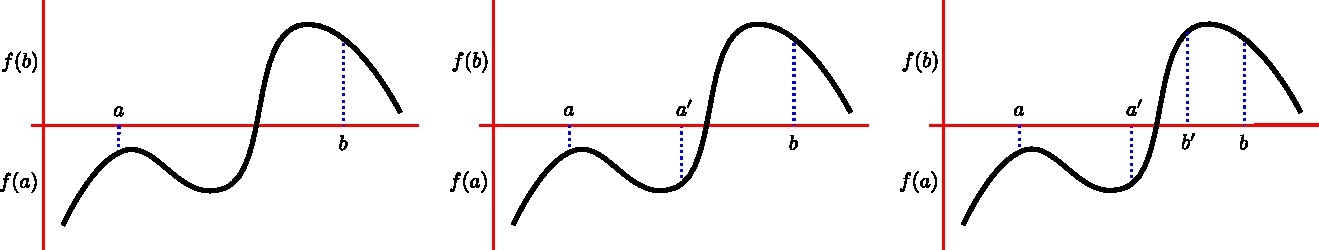
\includegraphics[width=\textwidth]{IVT3}
\end{center}
\end{fig}
Consider the leftmost of the above figures. It depicts a continuous function
that is negative at $x=a$ and positive at $x=b$. So choose $Y=0$ and apply the
IVT --- there must be some $c$ with $a \leq c \leq b$ so that $f(c) = Y = 0$.
While this doesn't tell us $c$ exactly, it does give us bounds on the possible positions
of at least one zero --- there must be at least one c obeying $a \le c \le b$.

See middle figure. To get better bounds we could test a point half-way between
$a$ and $b$. So set $a' = \frac{a+b}{2}$. In this example we see that $f(a')$
is
negative. Applying the IVT again tells us there is some $c$ between $a'$ and
$b$
so that $f(c) = 0$. Again --- we don't have $c$ exactly, but we have halved the
range of values it could take.

Look at the rightmost figure and do it again --- test the point half-way between
$a'$ and $b$. In this example we see that $f(b')$ is positive. Applying the IVT
tells us that there is some $c$ between $a'$ and $b'$ so that $f(c) = 0$. This
new range is a quarter of the length of the original. If we keep doing this
process the range will halve each time until we know that the zero is inside
some tiny range of possible values. This process is called the bisection method.

Consider the following zero-finding example
\begin{eg}\label{eg pre bisection}
Show that the function $f(x) = x-1+\sin(\pi x/2)$ has a zero
in $0 \leq x \leq 1$.

This question has been set up nicely to lead us towards using the IVT;  we are
already given a nice interval on which to look. In general we might have to
test a few points and experiment a bit with a calculator before we can
start narrowing down a range.

Let us start by testing the endpoints of the interval we are given
\begin{align*}
  f(0) &= 0 - 1 + \sin(0) = -1 < 0 \\
  f(1) &= 1-1+\sin(\pi/2) = 1 > 0
\end{align*}
So we know a point where $f$ is positive and one where it is negative. So by
the IVT there is a point in between where it is zero.

\emph{BUT} in order to apply the IVT we have to show that the function is
continuous, and we cannot simply write
\begin{quote}
 it is continuous
\end{quote}
We need to explain to the reader \emph{why} it is continuous. That is --- we
have to prove it.

So to write up our answer we can put something like the following ---
keeping in mind we need to tell the reader what we are doing so they can follow
along easily.
\begin{itemize}
\item We will use the IVT to prove that there is a zero in $[0,1]$.
\item First we must show that the function is continuous.
\begin{itemize}
\item Since $x-1$ is a polynomial it is continuous everywhere.
\item The function $\sin(\pi x/2)$ is a trigonometric function and is also
continuous everywhere.
\item The sum of two continuous functions is also continuous, so $f(x)$ is
continuous everywhere.
\end{itemize}
\item Let $a=0, b=1$, then
\begin{align*}
  f(0) &= 0 - 1 + \sin(0) = -1 < 0 \\
  f(1) &= 1-1+\sin(\pi/2) = 1 > 0
\end{align*}
\item The function is negative at $x=0$ and positive at $x=1$. Since the
function is continuous we know there is a point $c \in [0,1]$ so that $f(c) =
0$.
 \end{itemize}
Notice that though we have not used full sentences in our explanation here, we
are still using words. Your mathematics, unless it is very straight-forward
computation, should contain words as well as symbols.
\end{eg}
The zero is actually located at about $x=0.4053883559$.

The bisection method is really just the idea that we can keep repeating the above
reasoning (with a calculator handy). Each iteration will tell us the location of the zero
more precisely. The following example illustrates this.
\begin{eg}\label{eg bisection}
 Use the bisection method to find a zero of
\begin{align*}
  f(x) &= x-1+\sin(\pi x/2)
\end{align*}
that lies between $0$ and $1$.

So we start with the two points we worked out above:
\begin{itemize}
 \item $a=0, b=1$ and
\begin{align*}
  f(0) &= -1\\
  f(1) &= 1
\end{align*}
 \item Test the point in the middle $x = \frac{0+1}{2} = 0.5$
\begin{align*}
  f(0.5) &= 0.2071067813 > 0
\end{align*}
\item So our new interval will be $[0,0.5]$ since the function is negative at
$x=0$ and positive at $x=0.5$
\end{itemize}
Repeat
\begin{itemize}
 \item $a=0, b=0.5$ where $f(0)<0$ and $f(0.5)>0$.
 \item Test the point in the middle $x = \frac{0+0.5}{2} = 0.25$
\begin{align*}
  f(0.25) &= -0.3673165675 < 0
\end{align*}
\item So our new interval will be $[0.25,0.5]$ since the function is negative
at $x=0.25$ and positive at $x=0.5$
\end{itemize}
Repeat
\begin{itemize}
 \item $a=0.25, b=0.5$ where $f(0.25)<0$ and $f(0.5)>0$.
 \item Test the point in the middle $x = \frac{0.25+0.5}{2} = 0.375$
\begin{align*}
  f(0.375) &= -0.0694297669 < 0
\end{align*}
\item So our new interval will be $[0.375,0.5]$ since the function is negative
at $x=0.375$ and positive at $x=0.5$
\end{itemize}
Below is an illustration of what we have observed so far together with a plot of the
actual function.
\begin{efig}
 \begin{center}
  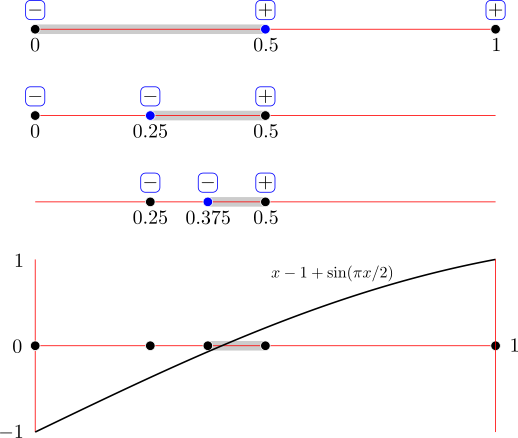
\includegraphics[width=\textwidth]{ivt_eg}
 \end{center}
\end{efig}

And one final iteration:
\begin{itemize}
 \item $a=0.375, b=0.5$ where $f(0.375)<0$ and $f(0.5)>0$.
 \item Test the point in the middle $x = \frac{0.375+0.5}{2} = 0.4375$
\begin{align*}
  f(0.4375) &= 0.0718932843>0
\end{align*}
\item So our new interval will be $[0.375,0.4375]$ since the function is
negative at $x=0.375$ and positive at $x=0.4375$
\end{itemize}
So without much work we know the location of a zero inside a range of length
$0.0625 = 2^{-4}$. Each iteration will halve the length of the range and we
keep going until we reach the precision we need, though it is much easier to
program a computer to do it.
\end{eg}

\section{(Optional) --- Making the Informal a Little More Formal}
\label{sec opt formal limit}
As we noted above, the definition of limits that we have been working with was
quite informal and not mathematically rigorous. In this (optional) section we
will work to understand the rigorous definition of limits.

Here is the formal definition --- we will work through it all very slowly and
carefully afterwards, so do not panic.
\begin{defn}\label{def_1_7_1}
 Let $a \in \mathbb{R}$ and let $f(x)$ be a function defined everywhere in a
neighbourhood of $a$, except possibly at $a$. We say that
\begin{quote}
 the limit as $x$ approaches $a$ of $f(x)$ is $L$
\end{quote}
or equivalently
\begin{quote}
 as $x$ approaches $a$, $f(x)$ approaches $L$
\end{quote}
and write
\begin{align*}
  \lim_{x \to a} f(x) &= L
\end{align*}
if and only if for every $\epsilon >0$ there exists $\delta>0$ so that
\begin{align*}
%  \text{if } 0<|x-a| < \delta \text{ then } |f(x) - L| <\epsilon.
  |f(x) - L| <\epsilon & \text{ whenever } 0<|x-a| < \delta
\end{align*}
Note that an equivalent way of writing this very last statement is
\begin{align*}
  \text{if } 0<|x-a| < \delta \text{ then } |f(x) - L| <\epsilon.
\end{align*}
\end{defn}
This is quite a lot to take in, so let us break it down into pieces.
\begin{defn}[The typical 3 pieces of a definition]\label{def_1_7_2}
Usually a definition can be broken down into three pieces.
 \begin{itemize}
  \item Scene setting --- define symbols and any
restrictions on the objects that we are talking about.
  \item Naming --- state the name and any notation for the property or object
that the definition is about.
  \item Properties and restrictions --- this is the heart of the definition
where we explain to the reader what it is that the object (in our case a
function) has to do in order to satisfy the definition.
 \end{itemize}
\end{defn}
Let us go back to the definition and look at each of these pieces in turn.
\begin{itemize}
 \item Setting things up --- The first sentence of the definition is really
just setting up the picture. It is telling us what the definition is about and
sorting out a few technical details.
\begin{itemize}
 \item \textbf{Let $a \in \mathbb{R}$} --- This simply tells us that the symbol
``$a$'' is a real number\footnote{The symbol ``$\in$'' is read as ``is an
element of'' --- it is definitely not the same as $e$ or $\epsilon$ or
$\varepsilon$. If you do not recognise ``$\mathbb{R}$'' or understand the
difference between $\mathbb{R}$ and $R$, then please go back and read Chapter~\ref{chap
basics} carefully.}.
 \item \textbf{Let $f(x)$ be a function} --- This is just setting the scene so
that we understand all of the terms and symbols.
 \item \textbf{defined everywhere in a neighbourhood of $a$, except possibly at
$a$} --- This is just a technical requirement; we need our function to be
defined in a little region\footnote{The term ``neighbourhood of $a$'' means a
small open interval around $a$ --- for example $(a-0.01, a+0.01)$. Typically
we don't really care how big this little interval is.} around $a$. The
function doesn't have to be defined everywhere, but it must be defined for all
$x$-values a little less than $a$ and a little more than $a$. The definition
does not care about what the function does outside this little window, nor does
it care what happens exactly at $a$.
\end{itemize}
\item Names, phrases and notation --- The next part of the definition is simply
naming the property we are discussing and tells us how to write it down. i.e. we
are talking about ``limits'' and we write them down using the symbols
indicated.
\item The heart of things --- we explain this at length below, but for now we
will give a quick explanation. \textbf{Work on these two points. They are hard.}
  \begin{itemize}
   \item \textbf{for all $\epsilon>0$ there exists $\delta >0$} --- It is
important we read this in order. It means that we can pick any positive number
$\epsilon$ we want and there will always be another positive number $\delta$
that is going to make what ever follows be true.
   \item \textbf{if $0<|x-a|<\delta$ then $|f(x)-L|<\epsilon$} --- From the
previous point we have our two numbers --- any $\epsilon >0$ then based on that
choice of $\epsilon$ we have a positive number $\delta$. The current statement
says that whenever we have chosen $x$ so that it is very close to $a$, then
$f(x)$ has to be very close to $L$. How close it ``very close''? Well
$0<|x-a|<\delta$ means that $x$ has to be within a distance $\delta$ of $a$
(but not exactly $a$) and similarly $|f(x)-L|<\epsilon$ means that $f(x)$ has
to
be within a distance $\epsilon$ of $L$.
  \end{itemize}
\end{itemize}
That is the definition broken up into pieces which hopefully now make more
sense, but what does it actually \emph{mean}? Consider a function we saw earlier
\begin{align*}
 f(x) &= \begin{cases}
          2x & x\neq3 \\
          9 & x=3
         \end{cases}
\end{align*}
and sketch it again:
\begin{fig}
\begin{center}
 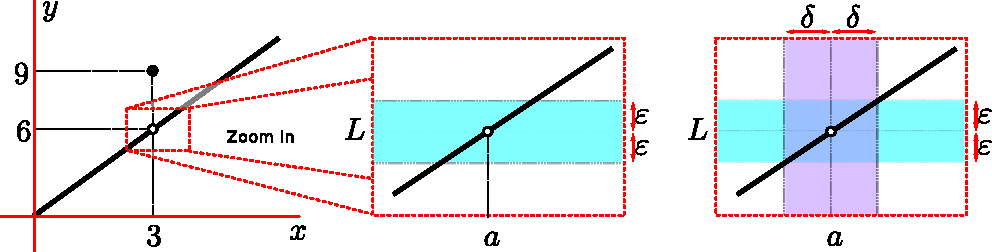
\includegraphics[width=\textwidth]{epsdelt1}
\end{center}
\end{fig}
We know (from our earlier work) that $\lim_{x \to 3} f(x) = 6$, so zoom in
around $(x,y)=(3,6)$. To make this look more like our definition, we have $a=3$
and $L=6$.
\begin{itemize}
 \item Pick some small number $\epsilon>0$ and highlight the horizontal strip
of all points $(x,y)$ for which $|y-L|<\epsilon$. This means all the
$y$-values have to satisfy $L-\epsilon < y < L+\epsilon$.

\item You can see that the graph of the function passes through this strip for
some $x$-values close to $a$. What we need to be able to do is to pick a
vertical strip of $x$-values around $a$ so that the function lies inside the
horizontal strip.

\item That is, we must find a small number $\delta>0$ so that for any $x$-value
inside the vertical strip $a-\delta < x < a+\delta$, \emph{except exactly at
$x=a$}, the value of the function lies inside the horizontal strip, namely
$L-\epsilon < y=f(x) < L+\epsilon$.

\item We see (pictorially) that we can do this. If we were to choose a
smaller value of $\epsilon$ making the horizontal strip narrower, it is clear
that we can choose the vertical strip to be narrower. Indeed, it
doesn't matter how small we make the horizontal strip, we will always be able
to construct the second vertical strip.
\end{itemize}

The above is a pictorial argument, but we can quite easily make it into a
mathematical one. We want to show the limit is $6$. That means for any
$\epsilon$ we need to find a $\delta$ so that when
\begin{align*}
  3-\delta < x < 3+\delta \text{ with $x \neq 3$} && \text{we have } &&
6-\epsilon < f(x) < 6+\epsilon
\end{align*}
Now we note that when $x \neq 3$, we have $f(x)=2x$ and so
\begin{align*}
  6-\epsilon < f(x) < 6+\epsilon && \text{implies that} &&
  6-\epsilon < 2x < 6+\epsilon
\intertext{this nearly specifies a range of $x$ values, we just need to divide
by $2$}
  3-\epsilon/2 < x < 3+\epsilon/2
\intertext{Hence if we choose $\delta = \epsilon/2$ then we get the desired
inequality}
  3-\delta < x < 3+\delta
\end{align*}
i.e. --- no matter what $\epsilon>0$ is chosen, if we put $\delta=\epsilon/2$
then when $3-\delta<x<3+\delta$ with $x \neq 3$ we will have $6-\epsilon < f(x)
< 6+\epsilon$. This is exactly what we need to satisfy the definition of
``limit'' above.

The above work gives us the argument we need, but it still needs to be written
up properly. We do this below.
\begin{eg}\label{eg_1_7_1}
Find the limit as $x \to 3$ of the following function
\begin{align*}
 f(x) &= \begin{cases}
          2x & x\neq 3 \\
          9 & x=3
         \end{cases}
\end{align*}
\begin{proof}
 We will show that the limit is equal to $6$. Let $\epsilon >0$ and $\delta =
\epsilon/2$. It remains to show that $|f(x)-6| <\epsilon$ whenever
$|x-3|<\delta$.

So assume that $|x-3|<\delta$, and so
\begin{align*}
  3-\delta < x < 3+\delta && \text{multiply both sides by 2} \\
  6-2\delta < 2x < 6+2\delta
\intertext{Recall that $f(x)=2x$ and that since $\delta=\epsilon/2$}
  6-\epsilon < f(x) < 6+\epsilon.
\end{align*}
We can conclude that $|f(x)-6| <\epsilon$ as required.
\end{proof}
\end{eg}

Because of the $\epsilon$ and $\delta$ in the definition of limits, we need to
have $\epsilon$ and $\delta$ in the proof. While $\epsilon$ and $\delta$ are
just symbols playing particular roles, and could be replaced with other symbols,
this style of proof is usually called $\epsilon$--$\delta$ proof.


In the above example everything works, but it can be very instructive to see
what happens in an example that doesn't work.
\begin{eg}\label{eg_1_7_2}
Look again at the function
\begin{align*}
  f(x) &= \begin{cases}
           x & x<2 \\
           -1 & x=2 \\
           x+3 & x>2
          \end{cases}
\end{align*}
and let us see why, according to the definition of the limit, that $\ds \lim_{x
\to 2} f(x) \neq 2$. Again, start by sketching a picture and zooming in around
$(x,y) = (2,2)$:
\begin{efig}
\begin{center}
 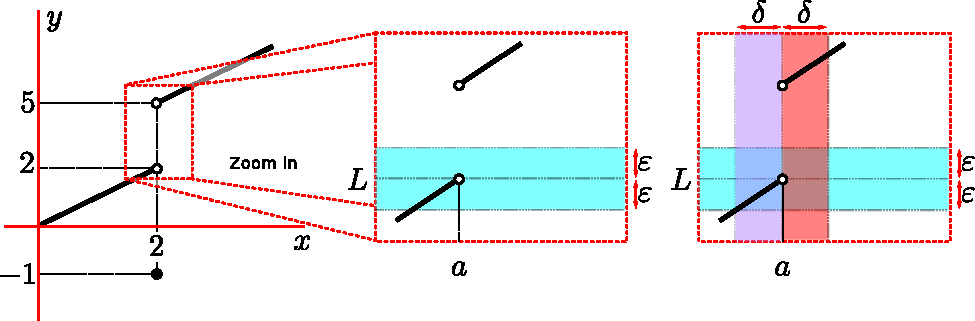
\includegraphics[width=\textwidth]{epsdelt2}
\end{center}
\end{efig}
Try to proceed through the same steps as before:
\begin{itemize}
 \item Pick some small number $\epsilon>0$ and highlight a horizontal
strip that  contains all $y$-values with $|y-L|<\epsilon$. This means all
the $y$-values have to satisfy $L-\epsilon < y < L+\epsilon$.

\item You can see that the graph of the function passes through this strip for
some $x$-values close to $a$. To the left of $a$, we can always find some
$x$-values that make the function sit inside the horizontal-$\epsilon$-strip.
However, unlike the previous example, there is a problem to the right of $a$.
Even for $x$-values just a little larger than $a$, the value of $f(x)$ lies
well
outside the horizontal-$\epsilon$-strip.

\item So given this choice of $\epsilon$, we can find a $\delta>0$ so that for
$x$ inside the vertical strip $a-\delta < x < a$, the value of the function sits
inside the horizontal-$\epsilon$-strip.

\item Unfortunately, there is no way to choose a $\delta>0$ so that for $x$
inside the vertical strip $a<x<a+\delta$ (with $x \neq a$) the value of the
function sits inside the horizontal-$epsilon$-strip.

\item So it is impossible to choose $\delta$ so that for $x$ inside the
vertical strip $a-\delta < x < a+\delta$ the value of the function sits inside
the horizontal strip $L-\epsilon < y=f(x) < L+\epsilon$.

\item Thus the limit of $f(x)$ as $x \to 2$ is not $2$.
\end{itemize}
\end{eg}

Doing things formally with $\epsilon$'s and $\delta$'s is quite painful for
general functions. It is far better to make use of the arithmetic of limits
(Theorem~\ref{thm arith lim}) and some basic building blocks (like those in
Theorem~\ref{thm easy lim}). Thankfully for most of the problems we deal with in
calculus (at this level at least) can be approached in exactly this way.

This does leave the problem of proving the arithmetic of limits and the limits
of the basic building blocks. The proof of the Theorem~\ref{thm arith lim} is
quite involved and we leave it to the very end of this Chapter. Before we do
that we will prove Theorem~\ref{thm easy lim} by a formal $\epsilon$--$\delta$
proof. Then in the next section we will look at the formal definition of limits
at infinity and prove Theorem~\ref{thm basic lim inf}. The proof of the
Theorem~\ref{thm arith inf lim}, the arithmetic of infinite limits, is very
similar to that of Theorem~\ref{thm arith lim} and so we do not give it.

So let us now prove Theorem~\ref{thm easy lim} in which we stated two simple
limits:
\begin{align*}
  \lim_{x \to a} c &= c & \text{ and } && \lim_{x \to a} x &= a.
\end{align*}
Here is the formal $\epsilon$--$\delta$ proof:
\begin{proof}[Proof of Theorem~\ref{thm easy lim}]
 Since there are two limits to prove, we do each in turn. Let $a,c$ be real
numbers.
\begin{itemize}
 \item Let $\epsilon>0$ and set $f(x)=c$. Choose $\delta=1$, then for any
$x$ satisfying $|x-a|<\delta$ (or indeed any real number $x$ at all) we have
$|f(x)-c| = 0 <\epsilon$. Hence $\ds \lim_{x \to a} c = c$ as required.

 \item Let $\epsilon>0$ and set $f(x)=x$. Choose $\delta=\epsilon$, then for
any $x$ satisfying $|x-a|<\delta$ we have
\begin{align*}
  a-\delta < x < a+\delta & \text{ but $f(x) = x$ and $\delta=\epsilon$ so} \\
  a-\epsilon < f(x) < a+\epsilon
\end{align*}
Thus we have $|f(x)-a|<\epsilon$. Hence $\ds \lim_{x \to a} x = a$ as required.
\end{itemize}
This completes the proof.
\end{proof}


\section{(Optional) --- Making Infinite Limits a Little More Formal}
\label{sec lim inf formal}
For those of you who made it through the formal $\epsilon-\delta$ definition of
limits we give the formal definition of limits involving infinity:
\begin{defn}[Limits involving infinity --- formal]\label{def_1_8_1}
\begin{enumerate}[(a)]
\item 
 Let $f$ be a function defined on the whole real line. We say that
\begin{quote}
  the limit as $x$ approaches $\infty$ of $f(x)$ is $L$
\end{quote}
or equivalently
\begin{quote}
 $f(x)$ converges to $L$ as $x$ goes to $\infty$
\end{quote}
and write
\begin{align*}
  \lim_{x \to \infty} f(x) &= L
\end{align*}
if and only if for every $\epsilon>0$ there exists $M \in \mathbb{R}$ so that
$|f(x)-L| < \epsilon$ whenever $x>M$.

Similarly we write
\begin{align*}
  \lim_{x \to -\infty} f(x) &= K
\end{align*}
if and only if for every $\epsilon>0$ there exists $N \in \mathbb{R}$ so that
$|f(x)-K| < \epsilon$ whenever $x<N$.

\item 
 Let $a$ be a real number and $f(x)$ be a function defined for all $x\ne a$.
We write
\begin{align*}
  \lim_{x \to a} f(x) &= \infty
\end{align*}
if and only if for every $P >0$  there exists $\delta>0$ so that
$f(x) > P$ whenever $0<|x-a|<\delta$.

\item 
Let $f$ be a function defined on the whole real line. We write
\begin{align*}
  \lim_{x \to \infty} f(x) &= \infty
\end{align*}
if and only if for every $P > 0$  there exists $M>0$ so that
$f(x) > P$ whenever $x>M$.

\end{enumerate}

\end{defn}
Note that we can loosen the above requirements on the domain of definition of $f$ --- for example, in part (a) all we actually require is that $f(x)$ be
defined for all $x$ larger than some value. It would be sufficient to 
require ``there is some $x_0 \in \mathbb{R}$ so that $f(x)$ is
defined for all $x>x_0$''. Also note that there are obvious variations of parts (b) and (c) with $\infty$ replaced by $-\infty$.

For completeness let's prove Theorem~\ref{thm basic lim inf} using this formal
definition. The layout of the proof will be very similar to our proof of
Theorem~\ref{thm easy lim}.
\begin{proof}[Proof of Theorem~\ref{thm basic lim inf}.]
There are four limits to prove in total and we do each in turn. Let $c \in
\mathbb{R}$.
\begin{itemize}
 \item Let $\epsilon>0$ and set $f(x)=c$. Choose $M=0$, then for any
$x$ satisfying $x>M$ (or indeed any real number $x$ at all) we have
$|f(x)-c| = 0 <\epsilon$. Hence $\ds \lim_{x \to \infty} c = c$ as required.
%%
\item The proof that $\ds \lim_{x \to -\infty} c = c$ is nearly identical.
Again, let $\epsilon>0$ and set $f(x)=c$. Choose $N=0$, then for any
$x$ satisfying $x<N$ we have $|f(x)-c| = 0 <\epsilon$. Hence $\ds \lim_{x \to
-\infty} c = c$ as required.
%%
\item Let $\epsilon>0$ and set $f(x)=x$. Choose $M = \frac{1}{\epsilon}$. Then
when $x>M$ we have
\begin{align*}
  0 < M & < x  & \text{divide through by $xM$ to get}\\
  0 < \frac{1}{x} & < \frac{1}{M} = \epsilon
\end{align*}
Since $x>0$, $\nicefrac{1}{x} = |\nicefrac{1}{x}| = |\nicefrac{1}{x} - 0| <
\epsilon$ as required.

\item Again, the proof in the limit to $-\infty$ is similar but we have to be
careful of signs. Let $\epsilon>0$ and set $f(x)=x$. Choose $N
= -\frac{1}{\epsilon}$. Then when $x< N$ we have
\begin{align*}
  0 > N & > x  &\text{ divide through by $xN$ to get}\\
  0 > \frac{1}{x} &> \frac{1}{N} = -\epsilon
\end{align*}
Notice that by assumption both $x,N<0$, so $xN>0$. Now since $x<0$,
$\nicefrac{1}{x} = -|\nicefrac{1}{x}| = |\nicefrac{1}{x} - 0| < \epsilon$ as
required.
\end{itemize}
This completes the proof.

\end{proof}

\section{(Optional) --- Proving the Arithmetic of Limits}\label{sec proof arith lim}


Perhaps the most useful theorem of this chapter is Theorem~\ref{thm arith lim}
which shows how limits interact with arithmetic. In this (optional) section we will prove both the arithmetic of limits Theorem~\ref{thm arith lim}
and the Squeeze Theorem~\ref{thm squeeze}. Before we get to the proofs it
is very helpful to prove three technical lemmas that we'll need. The
first is a very general result about absolute values of numbers:
\begin{lemma}[The triangle inequality]\label{lem_1_9_1}
 For any $x,y \in \mathbb{R}$
\begin{align*}
  |x+y| & \leq |x| + |y|
\end{align*}
\end{lemma}
\begin{proof}
Notice that for any real number $x$, we always have $-x,x\le|x|$ and either $|x|=x$
or $|x|=-x$. So now let  $x,y \in \mathbb{R}$. Then we must have either
\begin{alignat*}{3}
  |x+y|&= x+y &&\le |x|+|y|
\intertext{or}
  |x+y|&= -x-y &&\le |x|+|y|
\end{alignat*}
In both cases we end up with $|x+y| \le |x| + |y|$.
\end{proof}


The second lemma is more specialised. It proves that if we have a function
$f(x) \to F$ as $x \to a$ then there must be a small window around $x=a$ where
the function $f(x)$ must only take values not far from $F$. In particular it tells
us that $|f(x)|$ cannot be bigger than $|F|+1$ when $x$ is very close to $a$.
\begin{lemma}
\label{lem fx F1}
 Let $a \in \mathbb{R}$ and let $f$ be a function so that $\ds \lim_{x \to
a} f(x) =F$. Then there exists a $\delta >0$ so that if $0<|x-a|<\delta$
then we also have $|f(x)| \leq |F|+1$.
\end{lemma}
The proof is mostly just manipulating the $\epsilon$--$\delta$ definition of
a limit with $\epsilon=1$.
\begin{proof}
  Let $\epsilon = 1$. Then since $f(x) \to F$ as $x \to a$, there exists a
$\delta>0$ so that when $0<|x-a|<\delta$, we also have $|f(x)-F| \leq
\epsilon=1$. So now assume $0<|x-a|<\delta$. Then
\begin{align*}
  -\epsilon &\leq f(x) - F \leq \epsilon & \text{rearrange a little} \\
  -\epsilon+F &\leq f(x) \leq \epsilon+F
\intertext{Now $\epsilon+F \leq \epsilon+|F|$ and $-\epsilon+F \geq
-\epsilon-|F|$, so}
  -\epsilon-|F| &\leq f(x) \leq \epsilon+|F|
\end{align*}
Hence we have $|f(x)| \leq \epsilon+|F| = |F|+1$.
\end{proof}
Finally our third technical lemma gives us a bound in the other direction; it
tells us that when $x$ is close to $a$, the value of $|f(x)|$ cannot be much
smaller than $|F|$.
\begin{lemma}
\label{lem fx F2}
 Let $a \in \mathbb{R}$ and $F\ne0$ and let $f$ be a function so that $\ds \lim_{x \to a}
f(x) = F$. Then there exists $\delta>0$ so that when $0<|x-a|<\delta$, we have
$|f(x)|> \nicefrac{|F|}{2}$.
\end{lemma}
\begin{proof}
 Set $\epsilon = \nicefrac{|F|}{2}>0$. Then since $f(x) \to F$, we know there exists
a $\delta>0$ so that when $0<|x-a|<\delta$ we have $|f(x)-F|<\epsilon$. So now
assume $0<|x-a|<\delta$ so that $|f(x)-F|<\epsilon = \nicefrac{|F|}{2}$.  Then
\begin{align*}
  |F| &= |F-f(x)+f(x)| & \text{sneaky trick} \\
  & \leq |f(x) - F| + |f(x)| & \text{ but $|f(x)-F|<\epsilon$}\\
  & < \epsilon + |f(x)|
\end{align*}
Hence $|f(x)|>|F|-\epsilon= \nicefrac{|F|}{2}$ as required.
\end{proof}


Now we are in a position to prove Theorem~\ref{thm arith lim}. The proof has
more steps than the previous $\epsilon-\delta$ proofs we have
seen. This is mostly because we do not have specific functions $f(x)$ and
$g(x)$ and instead must play with them in the abstract --- and make good use of the
formal definition of limits.

We will break the proof into three pieces. The minimum that is required is to
prove that
\begin{align*}
  \lim_{x \to a} ( f(x) + g(x) ) &= F+G \\
  \lim_{x \to a} f(x) \cdot g(x) &= F\cdot G \\
  \lim_{x \to a} \nicefrac{1}{g(x)} &= \nicefrac{1}{G}\quad\text{if $G\ne 0$}.
\end{align*}
From these three we can prove that
\begin{align*}
  \lim_{x \to a} f(x) \cdot c &= F\cdot c \\
  \lim_{x \to a} ( f(x) - g(x) ) &= F-G \\
  \lim_{x \to a} \nicefrac{f(x)}{g(x)} &= \nicefrac{F}{G}\quad\text{if $G\ne 0$}.
\end{align*}
The first follows by setting $g(x) = c$ and using $\lim f(x) \cdot
g(x)$. The second follows by setting $c=-1$, putting $h(x) = (-1)\cdot g(x)$
and then applying both $\lim f(x) \cdot g(x)$ and $\lim f(x)+g(x)$. The third
follows by setting $h(x) = \nicefrac{1}{g(x)}$ and then using $\lim f(x) \cdot h(x)$.


Starting with addition, in order to satisfy the definition of limit, we are
going to have to show that
\begin{align*}
  |( f(x) + g(x) )-(F+G) | &\text{ is small}
\end{align*}
when we know that $|f(x)-F|, |g(x)-G|$ are small. To do this we use the
triangle inequality above showing that
\begin{align*}
  |( f(x) + g(x) )-(F+G) | &=
  |(f(x)-F) + (g(x)-G) | \leq |f(x)-F| + |g(x)-G|
\end{align*}
This is the key technical piece of the proof. So if we want the LHS of the
above to be size $\epsilon$, we need to make sure that each term on the RHS is
of size $\nicefrac{\epsilon}{2}$. The rest of the proof is setting up facts
based on the definition of limits and then rearranging facts to reach the
conclusion.
\begin{proof}{Proof of Theorem~\ref{thm arith lim} --- limit of a sum.}\ \ \
Let $a \in \mathbb{R}$ and assume that
\begin{align*}
  \lim_{x \to a} f(x) &= F & \text{ and } &&
  \lim_{x \to a} g(x) &= G.
\end{align*}
We wish to show that
\begin{align*}
\lim_{x \to a} f(x)+g(x) &= F+G.
\end{align*}

Let $\epsilon>0$ --- we have to find a $\delta>0$ so that when
$|x-a|<\delta$ we have $|(f(x)+g(x))-(F+G)|<\epsilon$.

Let $\epsilon>0$ and set $\epsilon_1 = \epsilon_2 = \nicefrac{\epsilon}{2}$.
By the definition of limits, because $f(x) \to F$ there exists some
$\delta_1 >0$ so that whenever $|x-a|<\delta_1$, we also
have $|f(x)-F|<\epsilon_1$. Similarly there exists $\delta_2>0$ so that if
$|x-a|<\delta_2$, then we must have $|g(x)-G|<\epsilon_2$. So now choose
$\delta = \min\{ \delta_1, \delta_2 \}$ and assume $|x-a|<\delta$. Then we must
have that $|x-a|<\delta_1, \delta_2$ and so we also have
\begin{align*}
  |f(x)-F|&<\epsilon_1 & |g(x)-G|& < \epsilon_2
\end{align*}

Now consider $|(f(x)+g(x))-(F+G)|$ and rearrange the terms:
\begin{align*}
  |(f(x)+g(x))-(F+G)| &= |(f(x)-F)+(g(x)-G)| & \text{ now apply triangle
inequality} \\
  &\leq |f(x)-F| + |g(x)-G| & \text{ use facts from above}\\
  & < \epsilon_1 + \epsilon_2 \\
  &= \epsilon.
\end{align*}

Hence we have shown that for any $\epsilon>0$ there exists some $\delta>0$ so
that when $|x-a|<\delta$ we also have $|(f(x)+g(x))-(F+G)|<\epsilon$. Which
is exactly the formal definition of the limit we needed to prove.
\end{proof}

Let us do similarly for the limit of a product. Some of the details of the
proof are very similar, but there is a little technical trick in the middle to
make it work. In particular we need to show that
\begin{align*}
  |f(x) \cdot g(x) - F\cdot G| & \text{ is small}
\end{align*}
when we know that $|f(x)-F|$ and $|g(x)-G|$ are both small. Notice that
\begin{align*}
  f(x) \cdot g(x) - F\cdot G
  &= f(x) \cdot g(x) - F\cdot G + \underbrace{ f(x)\cdot G - f(x) \cdot G
}_{=0} \\
  &= f(x)\cdot g(x)- f(x) \cdot G + f(x) \cdot G - F\cdot G \\
  &= f(x)\cdot( g(x)-G) + (f(x)-F)\cdot G
\end{align*}
So if we know $|f(x)-F|$ is small and $|g(x)-G|$ is small then we are done ---
except that we also need to know that $f(x)$ doesn't become really large near
$a$ --- this is exactly why we needed to prove Lemma~\ref{lem fx F1}.

As was the case in the previous proof, we want the LHS to be of size at most
$\epsilon$, so we want, for example,  the two terms on the RHS to be of size at most
$\nicefrac{\epsilon}{2}$. This means
\begin{itemize}
 \item we need $|G|\cdot|f(x)-F|$ to be of size at most $\nicefrac{\epsilon}{2}$, and
 \item we need $|g(x)-G|$ to be of size at most $\nicefrac{\epsilon}{2(|F|+1)}$
since we know that $|f(x)| \leq |F|+1$ when $x$ is close to $a$.
\end{itemize}

\noindent
Armed with these tricks we turn to the proofs.
\begin{proof}{Proof of Theorem~\ref{thm arith lim} --- limit of a product.}\ \ \
  Let $a \in \mathbb{R}$ and assume that
\begin{align*}
  \lim_{x \to a} f(x) &= F & \text{ and } &&
  \lim_{x \to a} g(x) &= G.
\end{align*}
We wish to show that
\begin{align*}
\lim_{x \to a} f(x)\cdot g(x) &= F\cdot G.
\end{align*}

Let $\epsilon>0$. Set $\epsilon_1 = \frac{\epsilon}{2(|G|+1)}$ (the extra $+1$
in the denominator is just there to make sure that $\epsilon_1$ is well--defined even if $G=0$),
and $\epsilon_2 = \frac{\epsilon}{2(|F|+1)}$. From this we establish the
existence of $\delta_1,  \delta_2, \delta_3$ which we need below.
\begin{itemize}
 \item By assumption $f(x) \to F$ so there exists $\delta_1>0$ so that whenever
$|x-a|<\delta_1$, we also have $|f(x)-F|<\epsilon_1$.
\item Similarly because $g(x) \to G$, there exists $\delta_2>0$
so that whenever $|x-a|<\delta_2$, we also have  $|g(x)-G|<\epsilon_2$.
\item By Lemma~\ref{lem fx F1} there exists $\delta_3>0$ so that whenever
$|x-a|<\delta_3$, we also have $|f(x)| \leq |F|+1$.
\end{itemize}

Let $\delta = \min\{\delta_1, \delta_2, \delta_3 \}$, assume $|x-a|<\delta$
and consider $|f(x) \cdot g(x) - F\cdot G|$. Rearrange the terms as we did
above:
\begin{align*}
 | f(x) \cdot g(x) - F\cdot G |
  &= |f(x)\cdot( g(x)-G) + (f(x)-F)\cdot G | \\
  & \leq |f(x)| \cdot |g(x)-G| + |G| \cdot |f(x)-F|
\end{align*}
By our three dot-points above we know that $|f(x)-F|<\epsilon_1$ and
$|g(x)-G|<\epsilon_2$ and $|f(x)| \leq |F|+1$, so we have
\begin{align*}
 | f(x) \cdot g(x) - F\cdot G |
  &< |f(x)| \cdot \epsilon_2 + |G| \cdot \epsilon_1 & \text{sub in $\epsilon_1,
\epsilon_2$ and bound on $f(x)$}\\
  &< (|F|+1) \cdot \frac{\epsilon}{2(|F|+1)} + |G|\cdot\frac{\epsilon}{2(|G|+1)}\\
  &\leq  \frac{\epsilon}{2} + \frac{\epsilon}{2} = \epsilon.
\end{align*}

Thus we have shown that for any $\epsilon>0$ there exists $\delta>0$ so that
when $|x-a|<\delta$ we also have $|f(x)\cdot g(x)-F\cdot G|<\epsilon$. Hence
$f(x)\cdot g(x) \to F\cdot G$.
\end{proof}

Finally we can prove the limit of a reciprocal. Notice that
\begin{align*}
  \frac{1}{g(x)} - \frac{1}{G} &= \frac{G-g(x)}{g(x) \cdot G}
\end{align*}
We need to show the LHS is of size at most $\epsilon$ when $x$ is close enough to $a$,
 so if $G-g(x)$ is small we are done --- except if $g(x)$ or $G$ are close to zero. By assumption
(go back and read Theorem~\ref{thm arith lim}) we have $G \neq 0$, and we know from
Lemma~\ref{lem fx F2} that $|g(x)|$ cannot be smaller than $\nicefrac{|G|}{2}$.
Together these imply that the denominator on the RHS cannot be zero and indeed must be
of magnitude at least $\nicefrac{|G|^2}{2}$. Thus we need $|G-g(x)|$ to be of size at most
$\epsilon \cdot \nicefrac{|G|^2}{2}$.
\begin{proof}{Proof of Theorem~\ref{thm arith lim} --- limit of a reciprocal.}\ \ \
 Let $\epsilon>0$ and set $\epsilon_1 = \epsilon|G|^2 \cdot \frac{1}{2}$. We
now use this and Lemma~\ref{lem fx F2} to establish the existence of $\delta_1,
\delta_2$.
\begin{itemize}
 \item Since $g(x) \to G$ we know that there exists $\delta_1>0$ so that when
$|x-a|<\delta_1$ we also have $|g(x)-G|<\epsilon_1$.
 \item By Lemma~\ref{lem fx F2} there exists $\delta_2$ so that when
$|x-a|<\delta_2$ we also have $|g(x)|>\nicefrac{|G|}{2}$. Equivalently,
when $|x-a|<\delta_2$ we also have $\left|\frac{G}{2g(x)}\right|<1$.
\end{itemize}


Set $\delta = \min\{\delta_1,\delta_2\}$ and assume $|x-a|<\delta$. Then
\begin{align*}
  \left| \frac{1}{g(x)} - \frac{1}{G} \right|
  &= \left| \frac{G - g(x)}{g(x) \cdot G} \right| \\
  &= |g(x) - G| \cdot \frac{1}{|G|\cdot |g(x)|} & \text{ by assumption}
\\
  & < \frac{\epsilon_1}{|G| \cdot |g(x)|} & \text{ sub in $\epsilon_1$} \\
  & = \epsilon \cdot \frac{|G|}{2  |g(x)|} & \text{ since
$\left|\frac{G}{2g(x)}\right|<1$}\\
  & < \epsilon
\end{align*}
Thus we have shown that for any $\epsilon>0$ there exists $\delta>0$ so that
when $|x-a|<\delta$ we also have $|\nicefrac{1}{g(x)} -
\nicefrac{1}{G}|<\epsilon$. Hence $\nicefrac{1}{g(x)} \to \nicefrac{1}{G}$.
\end{proof}

\begin{proof}{Proof of Theorem~\ref{thm squeeze} --- Squeeze / sandwich / pinch.}\ \ \
In the squeeze theorem, we are given three functions $f(x)$, $g(x)$ and $h(x)$
and are told that
\begin{align*}
    f(x) \leq g(x) \leq h(x) \quad\text{and}\quad
    \lim_{x \to a} f(x) &= \lim_{x \to a} h(x) = L
\end{align*}
and we must conclude from this that $\lim\limits_{x \to a} g(x) = L$ too.
That is, we are given some fixed, but unspecified, $\epsilon>0$
and it is up to us to find a $\delta>0$ with the property that
$\left| g(x) - L \right|<\epsilon$ whenever $|x-a|<\delta$. Now because we have been told that $f$ and $h$ both converge to $L$, there exist $\delta_1>0$ and
$\delta_2>0$ such that
\begin{itemize}
 \item $\left| f(x) - L \right|<\epsilon$,\ \
           i.e. $L-\epsilon<f(x)<L+\epsilon$,\ \
           whenever $|x-a|<\delta_1$, and
 \item $\left| h(x) - L \right|<\epsilon$,\ \
           i.e. $L-\epsilon<h(x)<L+\epsilon$,\ \
           whenever $|x-a|<\delta_2$
\end{itemize}
So set $\delta = \min\{\delta_1,\delta_2\}$ and assume $|x-a|<\delta$. Then
both $L-\epsilon<f(x)<L+\epsilon$ and $L-\epsilon<h(x)<L+\epsilon$ so that
\begin{align*}
L-\epsilon<f(x) &\le g(x) \le h(x) < L+\epsilon & \text{which implies that}\\
L-\epsilon< & g(x) < L+\epsilon & \text{which in turn gives us}\\
&\left| g(x) - L \right|<\epsilon
\end{align*}
as desired.
\end{proof}
